\documentclass[english]{sareport}
% use the option peerreview for creating an anonymized version of your report
% E.g., \documentclass[english,peerreview]{sareport}

\usepackage[colorlinks, linkcolor=black, citecolor=black, urlcolor=black]{hyperref}
\usepackage{fontawesome}
\usepackage[normalem]{ulem}

\usepackage{graphicx}
\usepackage{rotating}
\usepackage{float}
\usepackage{enumitem}

\setlist{noitemsep} % \setlist{nosep}
\setlength{\parindent}{0pt}

% Set all authors, if your group counts 2, set third author empty \authorthree{}
% Set the groupname as well
\authorone{Monika Filipcikova (r0683254)}
\authortwo{Armin Halilovic(r0679689)}
\authorthree{}
\groupname{Filipcikova-Halilovic}
\academicyear{2016--2017}

\casename{Shared Internet Of Things Infrastructure Platform}
\phasenumber{2b}
\phasename{The Complete Architecture}

\begin{document}
\maketitle

\tableofcontents
% the following two command are necessary for obtaining the mini list of figures in the cs-view, decomposition view, deployment view and scenarios chapters
\dominilof
\fakelistoffigures

\chapter{Introduction}\label{ch:introduction}
"Since you are a two-student group, you can omit/disregard the low-priority
non-functional requirements (i.e., P2, U1, M2). Please make sure all other
elements of the assignment are provided."\\

Changes to decompositions 1 and 2.


\chapter{Architectural Decisions}\label{ch:overview}
    % \chapter{Architectural Decisions}\label{ch:overview}

\section{Av1: Communication between SIoTIP gateway and Online Service}

    \todoinline{Use this section structure for each requirement}

    \subsection*{Key Decisions}

        The \texttt{OnlineServiceMonitor} monitors the Gateway's connectivity to the Online Service.
        The \texttt{OnlineServiceBrokerMonitor} monitors the communication component on Gateways.

        \begin{itemize}
        	\item decision 1
        	\item \ldots
        \end{itemize}
        \emph{Employed tactics and patterns:} heartbeats, ping/echo


    \subsection*{Rationale}
        \paragraph{Av1: New Gateway responsibilities}
            The SIoTIP gateway is able to autonomously detect failures of its individual internal communication components.\\
            The Online Service should acknowledge each message sent by the SIoTIP gateway so that the gateway can detect failures.\\
            If an internal SIoTIP gateway component fails, the gateway first tries to restart the affected component.
            If the failure persists, the SIoTIP gateway reboots itself entirely. Note that the SIoTIP gateway,
            due to the occurred failure, cannot contact a system administrator itself.\\
            If (an internal communication component of) the Online Service or the communication
            channel has failed, the SIoTIP gateway will temporarily store all incoming pluggable data
            and any issued application commands internally.\\
            If the Online Service becomes unreachable, application parts running locally on the SIoTIP
            gateway continue to operate normally.\\
            The SIoTIP gateway will start synchronising with the Online service within 1 minute after the
            communication channel becomes available.\\
        
            The \texttt{OnlineServiceBroker} isolates communication-related concerns between Gateways and the Online Service
            along with GatewayBroker on the Online Service.Forwards requests from one party to the other and transmits results and 
            possible exceptions.
            The SIoTIP gateway is able to autonomously detect failures of its individual internal communication components.
            The  \texttt{OnlineServiceBrokerMonitor} monitors the communication component on Gateways. 
            If the communication component fails, the monitor tries to restart it. If the failure persists, 
            the gateway reboots itself entirely.\\
            The \texttt{BrokerLogic} handles all functionality related to communication. In the \texttt{OnlineServiceBroker} 
            are \texttt{RequestStore} and \texttt{OnlineServiceMonitor}. 

            The \texttt{OnlineServiceMonitor} monitors the Gateway's connectivity to the Online Service. It checks acknowledgement of each
            message sent by the SIoTIP gateway. If (an internal communication component of) the Online Service or the communication
            channel has failed, all requests to the Online Service will be stopped and stored in the \texttt{RequestStore}. An explicit command for this is not necessary,
            because the requests in the \texttt{RequestStore} will not be deleted, since no acknowledgements are received
            anymore from the Online Service. It can store at least 3 days of pluggable data before old data has to be overwritten. 
            After the monitor detects that a connection to the Online Service is possible
            again, it makes the gateway start synchronising again. When the Online Service is unreachable, application 
            parts running locally on the SIoTIP gateway continue to operate normally.
            
            
        \paragraph{Av1: New Online Service responsibilities}
            The Online Service is able to autonomously detect failures of its individual internal communication components.\\
            The Online Service is able to detect that a SIoTIP gateway is not sending data anymore based on the expected synchronisation interval.\\
            The Online Service notifies the infrastructure manager and a SIoTIP system administrator when the outage of a SIoTIP gateway is detected.\\
            The failure of an internal SIoTIP Online Service component is detected within 30 seconds.\\
            The detection time for a failed SIoTIP gateway or channel depends on the transmission rate
            of the gateway. An outage is defined as 3 consecutive expected synchronisations that do not
            arrive within 1 minute of their expected arrival time.\\
            The infrastructure owner is notified within 5 minutes after the detection of an outage of their gateway.\\
            A SIoTIP system administrator should be notified within 1 minute after the detection
            of a simultaneous outage of more than 1\% of the registered gateways.\\

            GatewayBroker: Isolates communication-related concerns between the Online Service Gateways and along with OnlineServiceBroker on Gateways.
                       Forwards requests from one party to the other and transmits results and possible exceptions. \\
                       Sends acknowledgements for all messages sent by Gateways so that they can detect failures.
            GatewayBrokerMonitor: Monitor the communication component for communication with gateways on the Online Service.

            In GatewayBroker:
                BrokerLogic: Handles all functionality related to communication.
                GatewayMonitor: Monitors the connectivity status all gateways. Can detect that a gateway is not sending data anymore based on the expected synchronisation interval. If 3 consecutive expected synchronisations do not arrive within 1 minute of their expected arrival time,
                            this is detected as a gateway outage. When outages of gateways are detected, the infrastructure owners that own the gateways and a SIoTIP system administrator are notified.
                            When the connectivity status change of a Gateway is detected, this is saved in the DeviceDB.



    \subsection*{Considered Alternatives}
         Alternative for monitoring of gateways:
        Gateway updated come to GatewayMonitor
        We could make GatewayMonitor ping all the gateways
        However, this would increase traffic on the network

    \subsection*{Deployment Decisions}
        OnlineServiceBroker
        OnlineServiceBrokerMonitor

        GatewayBroker
        GatewayBrokerMonitor

        For both the Online Service and Gateways, the components used for communication
        (\texttt{OnlineServiceBroker}, \texttt{GatewayBroker}) are to be deployed on different nodes than
        their monitoring components (\texttt{OnlineServiceBrokerMonitor}, \texttt{GatewayBrokerMonitor}).
        Otherwise, if the node of a communication
        component fails, its monitoring component would also fail and thus
        nothing would be detected.

    \subsection*{Considered Deployment Alternatives}
        \ldots

\newpage
\section{Av2: Application failure}

    \subsection*{Key Decisions}

        \begin{itemize}
        	\item \texttt{ApplicationInstance}s are executed within \texttt{ApplicationContainer}s.
            \item \texttt{ApplicationContainerManager} creates/destroys/handles communication for \texttt{ApplicationContainer}s.
            \item \texttt{ApplicationContainerMonitor} monitors \texttt{ApplicationContainer}s and \texttt{ApplicationInstance}s.
            \item \texttt{ApplicationExecutionSubsystemMonitor} monitors the application execution subsystem.
        \end{itemize}
        \emph{Employed tactics and patterns:} container

    \subsection*{Rationale}
        To handle Av2, we developed the whole application execution subsystem in a decomposition
        with Av2 and important application instance related use cases. The application execution subsystem
        is composed of the following components:
        \begin{itemize}
            \item \texttt{ApplicationContainer}
            \item \texttt{ApplicationContainerMonitor}
            \item \texttt{ApplicationContainerManager}
            \item \texttt{ApplicationExecutionSubsystemMonitor}
            \item \texttt{DeviceDataConverter}
            \item \texttt{DeviceCommandConstructor}
        \end{itemize}

        Av2 states "The system is able to autonomously detect failures of its individual
        application execution components, failing applications, and failing application containers.".\\
        These responsibilities are handled by the \texttt{ApplicationContainer}, \texttt{ApplicationContainerMonitor}, and \texttt{ApplicationExecutionSubsystemMonitor}.
        The \texttt{ApplicationContainer} provides a sandbox environment for an \texttt{ApplicationInstance} to run in and has the ability
        to monitor the instance. When an application instance fails, the container notifies the \texttt{ApplicationContainerMonitor} of this.\\
        Next to this, the \texttt{ApplicationContainerMonitor} pings \texttt{ApplicationContainer}s regularly to check whether or not the container
        has failed. If a failure of an application instance/container is detected, the \texttt{ApplicationContainerMonitor} sends a command to the
        \texttt{ApplicationContainerManager} to restart the instance/container or to create a new one in case the first two restarts did not work.
        If the application instance then keeps failing, it is suspended and the application provider and affected customer organisation are notified.
        When an application fails, a message of this is sent to the other parts of the application, so that they can possible run in a degraded mode. \\
        The \texttt{ApplicationContainerMonitor} also keeps track of how many times an \texttt{ApplicationInstance} has failed, so that when the container
        fails, there also is data about the instance.\\
        Lastly, the \texttt{ApplicationExecutionSubsystemMonitor} monitors other parts of the application execution subsystem, and restarts them
        in case failure is detected. \\

        Because of how different \texttt{ApplicationInstance}s run each in their own \texttt{ApplicationContainer}, no other applications or availability
        of other functionality of the system is affected.

    \subsection*{Deployment Decisions}
        For Av2, is important that \texttt{ApplicationInstance}s are deployed on different node from the \texttt{ApplicationContainerMonitor} that is responsible for
        monitoring. If the node the \texttt{ApplicationInstance} fails, then the \texttt{ApplicationContainerMonitor} won't also automatically fail with the \texttt{ApplicationInstance}
        and interested parties can be informed. \\
        In order to make sure that no applications or functionality of the system is affected when an application instance/container fails, each \texttt{ApplicationContainer}
        runs on its own node. The \texttt{ApplicationContainerManager} keeps track of all \texttt{ApplicationContainer}s.

\newpage
\section{Av3: Pluggable device or mote failure}

    \todoinline{Use this section structure for each requirement}

    \subsection*{Key Decisions}

    \todoinline{
    	Briefly list your key architectural decisions.
    	Pay attention to the solutions that you employed (in your own terms or using tactics and/or patterns).
    }

    \begin{itemize}
    	\item \texttt{DeviceManager} monitors connected/operational devices on a gateway.
    	\item \texttt{DeviceManager} stores the requirements for pluggable devices set by applications
    \end{itemize}
    \emph{Employed tactics and patterns:} heartbeat, ping/echo

    \subsection*{Rationale}
        \paragraph{Failure detection}
            Gateway need to be able to autonomously detect failure of one of its
            connected motes and pluggable devices. This is achieved by making motes
            send heartbeats to their connected gateways. The gateways can
            then monitor their connected devices. The heartbeats contain a list
            of devices that are connected/operational at the moment the mote sends
            the heartbeat. Each gateway makes use of a \texttt{DeviceManager}
            component to monitor the devices. This component uses timers to keep track
            of how long it has been since a device has sent a heartbeat or occured in
            a list of connected devices. Once a timer expires, this is treated as
            a failure. \\

            A mote has failed when 3 consecutive heartbeats do not arrive within 1
            second of their expected arrival time. \\
            A pluggable device has failed when it does not occur in a heartbeat of the
            mote in which it is expected to be in. This is is detected within 2
            seconds after the arrival of the heartbeat.

        \paragraph{Automatic application deactivation and redundancy settings}
            Applications should be automatically suspended when they can no longer
            operate due to failure of a pluggable device or mote and reactivated
            once the failure is resolved. Application providers can design their
            applications such that they explicitly require redundancy in
            the available pluggable devices. \\
            This problem is tackled by the \texttt{DeviceManager}. It
            stores the requirements for pluggable devices set by applications for all
            applications that use the gateway that the \texttt{DeviceManager}
            runs on. When it detects that an application can no longer operate
            due to failures, it will send a command to the \texttt{ApplicationManager}
            (via the \texttt{GatewayFacade})
            to suspend that application. When the required devices are operational
            again, the \texttt{DeviceManager} detects this and sends a
            command to reactivate the application. \\

            Applications are suspended within 1 minute after detecting
            the failure of an essential pluggable device. \\
            Application are reactivated within 1 minute after the failure is resolved.

        \paragraph{Notifications}
            The infrastructure owner should be notified of any persistent
            pluggable device or mote failures. Customer organisations should be
            notified if one or more of their applications is suspended or
            reactivated. Applications using a failed pluggable device or any device
            on a failed mote should be notified. \\
            The \texttt{NotificationHandler} was put in place to deal with
            notifications. Other components can use it to generate notifications for
            certain users in the system. The \texttt{NotificationHandler} will then
            insert information relevant to the notification in the database (message,
            status, date and time, source, ...), and use an external delivery
            service to deliver the notification to users. The used delivery medium
            is based on the user's preferences. The \texttt{DeviceManager} sends request
            to the external delivery service to notifies the
            infrastructure owner, once mote or pluggable device failure occurs.
            Since they are stored in the database, users can always view
            their notifications via their dashboard. However, this funcionality is not
            expanded on in this decomposition yet. \\

            Infrastructure owners are notified within 1 minute after detecting a mote outage lasting at
            least 10 seconds. \\
            Infrastructure owners are notified within 1 minute after the detection of the unavailability of
            a pluggable device for 30 seconds. \\
            Applications are notified of the failure of relevant pluggable devices within 10 seconds.


    \subsection*{Considered Alternatives}
        \paragraph{Alternative for failure detection}
            An alternative would have been to move the \texttt{DeviceManager}
            component from gateways to the Online Service. This solution would make the
            gateways do less work, but would be very unscalable. The reason is
            that as the customer base (and thus the amount of devices) increases,
            the Online Service would need to keep track of huge amounts of devices.
            This would also flood the network to the Online Service with heartbeats.

        \paragraph{Alternative for Failure detection}
            Another alternative for failure detection could have been the use of
            a Ping/Echo mechanism instead of Heartbeats. Pings could then be used
            to check if a device is currently operational. However, as a device could
            not be operational for a moment because of e.g. interference, timers
            would still be necessary to keep track of operational devices. We opted
            to use heartbeats, as this would reduce the amount of data sent over
            the network used by the motes, and as motes would have to do slightly
            more work to process each Ping request in order to generate a reply.

        \paragraph{Av3: Notifications}
            Reliable and quick delivery of notifications is crucial to the
            system in order to solve problems should things go wrong. Currently,
            the solution is to use a third party service for delivery of
            notifications. In the case that no external services are found
            satisfactory, or if this dependency on an external service is
            unwanted, it is possible to build an internal solution for this.
            For example, a \texttt{NotificationSender} component could make use
            of the \texttt{Factory pattern} for different message channels for
            different delivery methods (each with their own sendNotification method).
            This solution allows us to easily add new message channels in the
            future with little effort. The disadvantage of this is that an
            internal solution takes a lot more time to implement.


    \subsection*{Deployment Decisions}
        For Av3 is important that the \texttt{DeviceManager} is deployed on another node as the
        \texttt{Mote} and the \texttt{PluggableDevice}. The \texttt{DeviceManager}
        checks the \texttt{Mote} and the \texttt{PluggableDevice} availability and in case of failure, the \texttt{DeviceManager}
        can notify the infrastructure owner of any persistent pluggable device or mote failures.\\

\newpage
\section{M1: Integrate new sensor or actuator manufacturer}

    \subsection*{Key Decisions}

    \begin{itemize}
    	\item Modifiability is maintained by splitting up functionality that would need to be updated
              when new pluggable devices are introduced to the system into different components.
        \item In interfaces, pluggable devices are only referred to by their unique PluggableDeviceID,
              types and other device info is left out of parameter lists.
              
    \end{itemize}
    \emph{Employed tactics and patterns:} None

    \subsection*{Rationale}
        \paragraph{M1: Data conversion}
            With new types of devices, the pluggable data processing subsystem
            should be extended with relevant data conversions,
            e.g. converting temperature in degrees Fahrenheit to degrees Celsius. \\
            The \texttt{DeviceDataConverter} is put in place to handle the
            task of converting pluggable device data to data of a different type in the system.
            This component can easily be modified for new types of data simply by
            adding a new conversion method for the new.

        \paragraph{M1: Usage of new data by applications}
            The available applications in the system can be updated to use any
            new pluggable devices. \\
            This is made possible by the RequestData
            interface provided by \texttt{DeviceDataScheduler}.
            Data of the new type of device can be requested in the same way
            as for older devices: by using the device's unique id.
            The application manager can get pluggable device data from the
            \texttt{PluggableDeviceDataDB} and return this data to applications in
            the DeviceData datatype. This datatype can easily be
            updated for new types of pluggable devices.

        \paragraph{P2: Scheduling}
            The pluggable data processing subsystem needs to be able to run in normal
            or overload mode, depending on whether or not the system can process
            requests within the deadlines given in the quality requirement. Also,
            a mechanism should be in place to avoid starvation of any type of request. \\
            The \texttt{DeviceDataScheduler} is used to deal with this problem.
            It is responsible for scheduling requests that wish to interact with
            the \texttt{PluggableDeviceDataDB}. In normal mode, the system processes
            incoming requests in a FIFO order. In overload mode, the requests are
            given a priority based on what the request is for and what the source
            of the request is. The requests are then not simply processed in an
            order based on their priorities, but an aging technique is to be used
            such that starvation will be avoided. Thus, in overload mode,
            requests are processed in an order based on a combination of the
            priorities of the requests and the age of the requests.

        \paragraph{P2: Pluggable data separation}
            The processing of (large amounts of) requests concerning pluggable
            data has no impact on requests concerning other data, e.g. available applications. \\
            In order to statisfy this constraint, all data directly related to
            pluggable data has been separated into the \texttt{PluggableDeviceDataDB}.
            All requests concerning pluggable data will be handled by this new
            component. \texttt{PluggableDeviceDataDB} will run on a node different
            from the node that the \texttt{Datbase} component runs on. This way
            requests concerning pluggable will have no impact on
            requests concerning other data.

        \paragraph{M1: Handling new types of pluggable devices}
            The new types of sensor or actuator data should be transmitted,
            processed and stored, and should be made available to applications.
            The infrastructure managers must be able to initialize the new type
            of pluggable device, configure access rights for these devices, and
            view detailed information about the new type of pluggable device. \\
            The components created thus far have been created with high cohesion in
            mind so that updating them for new devices would be relatively straightforward.
            In order for this constraint to be satisfied, changes have to be made to
            the following elements:
            \begin{itemize}
                \item \emph{PluggableDevice}: This component needs to be updated
                      so that the new type of device can be initialised and configured,
                      and thus so that the device's data can be sent to the system.
                \item \emph{DeviceData}: Depending on how this data type
                      is implemented, it might need an update in order for it
                      to represent possible new data types (for example
                      Temperature Filipcikova) and for the new data types to be
                      serialized.
                \item \emph{PluggableDeviceDataDB}: The database needs to be updated
                      so that information can be retrieved about the new types
                      of sensors and the new types of data. Data related to the
                      displaying of sensor data will also need to be updated.
                \item \emph{PluggableDeviceConverter}: see above.
            \end{itemize}

    \subsection*{Considered Alternatives}
        \paragraph{Alternative(s) for choice 1} Explain what alternative(s) you
        considered for this design choice and why they where not selected.

    \subsection*{Deployment Decisions}
        \ldots

    \subsection*{Considered Deployment Alternatives}
        \ldots

\newpage
\section{P1: Large number of users}
    \todoinline{Use this section structure for each requirement}
    \subsection*{Key Decisions}
    \todoinline{
    	Briefly list your key architectural decisions.
    	Pay attention to the solutions that you employed (in your own terms or using tactics and/or patterns).}
    \begin{itemize}
    	\item decision 1
    	\item \ldots
    \end{itemize}
    \emph{Employed tactics and patterns:} \ldots

    \subsection*{Rationale}
    \todoinline{Describe the design choices related to \emph{ReqX} together with the rationale
    	of why these choices where made.}

    \subsection*{Considered Alternatives}
    \paragraph{Alternative(s) for choice 1} Explain what alternative(s) you
    considered for this design choice and why they where not selected.

    \subsection*{Deployment Decisions}
    \ldots

    \subsection*{Considered Deployment Alternatives}
    \ldots


\newpage
\section{P2: Requests to the pluggable data database}

    \subsection*{Key Decisions}

        \begin{itemize}
            \item \texttt{PluggableDeviceDataDB} separates the requests concerning pluggable data
                  so that those requests have no impact on requests concerning other data.
        	\item \texttt{DeviceDataScheduler} handles all requests for the \texttt{PluggableDeviceDataDB},
                  recognizes when the data processing subsystem needs to run in normal or overload mode,
                  and prevents starvation of requests.
        \end{itemize}
        \emph{Employed tactics and patterns:} \ldots

    \subsection*{Rationale}
        \paragraph{P2: Scheduling}
            The pluggable data processing subsystem needs to be able to run in normal
            or overload mode, depending on whether or not the system can process
            requests within the deadlines given in the quality requirement. Also,
            a mechanism should be in place to avoid starvation of any type of request. \\
            The \texttt{PluggableDeviceDataScheduler} is used to deal with this problem.
            It is responsible for scheduling requests that wish to interact with
            the \texttt{PluggableDeviceDB}. In normal mode, the system processes
            incoming requests in a FIFO order. In overload mode, the requests are
            given a priority based on what the request is for and what the source
            of the request is. The requests are then not simply processed in an
            order based on their priorities, but an aging technique is to be used
            such that starvation will be avoided. Thus, in overload mode,
            requests are processed in an order based on a combination of the
            priorities of the requests and the age of the requests.

        \paragraph{P2: Pluggable data separation}
            The processing of (large amounts of) requests concerning pluggable
            data has no impact on requests concerning other data, e.g. available applications. \\
            In order to statisfy this constraint, all data directly related to
            pluggable data has been separated into the \texttt{PluggableDeviceDB}.
            All requests concerning pluggable data will be handled by this new
            component. \texttt{PluggableDeviceDB} will run on a node different
            from the node that the \texttt{Datbase} component runs on. This way
            requests concerning pluggable will have no impact on
            requests concerning other data.

    \subsection*{Considered Alternatives}
        \paragraph{Alternative(s) for choice 1} Explain what alternative(s) you
        considered for this design choice and why they where not selected.

    \subsection*{Deployment Decisions}
        \ldots

    \subsection*{Considered Deployment Alternatives}
        \ldots

\newpage
\section{U2: Easy installation}

    \todoinline{Use this section structure for each requirement}

    \subsection*{Key Decisions}

        \todoinline{
        	Briefly list your key architectural decisions.
        	Pay attention to the solutions that you employed (in your own terms or using tactics and/or patterns).
        }

        \begin{itemize}
        	\item decision 1
        	\item \ldots
        \end{itemize}
        \emph{Employed tactics and patterns:} \ldots

    \subsection*{Rationale}
        \todoinline{
            Describe the design choices related to \emph{ReqX} together with the rationale
        	of why these choices where made.
        }

    \subsection*{Considered Alternatives}
        \paragraph{Alternative(s) for choice 1} Explain what alternative(s) you
        considered for this design choice and why they where not selected.

    \subsection*{Deployment Decisions}
        \ldots

    \subsection*{Considered Deployment Alternatives}
        \ldots


\section{Other decisions}

    \subsection{Authentication}
        \subsubsection*{KeyDecisions}
            A database is used to store login sessions.

        \subsubsection*{Rationale}
            Authentication is done by verifying user credentials when a user wants to log in. Then a unique session
            is created and the sessionID of this session is returned to the client used by the user. In all subsequent requests,
            the user's client adds this sessionID with the request. If the sessionID exists in the database, then this means
            that the user is still logged in and the request can be handled. Every time the sessionID is checked in the database,
            a timestamp is reset. After a certain time without any requests for this sessionID, the session is deleted from the system. \\

            The \texttt{SessionDB} is used to store all sessions.

        \subsubsection*{Considered Alternatives}
            \paragraph{Files for sessions}
                The sessions could be stored as files on the UserFacade that handlers requests for a user. The facade could then check
                whether or not a certain file exists to check if a user is logged in. However, this would make the facades stateful and
                would add extra overhead in keeping the session files on different nodes consistent with each other in case that the
                user is redirected to another node for load balancing. Keeping different nodes for facades consistent is much easier
                if they are all stateless.

        \subsubsection*{Deployment Decisions}
            The \texttt{SessionDB} is to be deployed on a separate node in order to avoid puttting extra strain on the other databases.
            We expect the SessionDB to receive many more requests than e.g. the \texttt{OtherDataDB}, since users need to send a sessionID
            with every request so that it can be checked whether or not the user is (still) logged in.

    \subsection{Notifications}
        \subsubsection*{KeyDecisions}
            The NotificationHandler stores and sends notifications.

        \subsubsection*{Rationale}
            The \texttt{NotificationHandler} was put in place to deal with
            notifications. Other components can use it to generate notifications for
            certain users in the system. The \texttt{NotificationHandler} will then
            insert information relevant to the notification in the database (message,
            status, date and time, source, ...), and use an external delivery
            service to deliver the notification to users. The used delivery medium
            is based on the user's preferences. The \texttt{DeviceManager} sends request
            to the external delivery service to notifies the
            infrastructure owner, once mote or pluggable device failure occurs.
            Since they are stored in the database, users can always view
            their notifications via their dashboard. \\

        \subsubsection*{Considered Alternatives}
            \paragraph{Custom delivery solution}
                Reliable and quick delivery of notifications is crucial to the
                system in order to solve problems should things go wrong. Currently,
                the solution is to use a third party service for delivery of
                notifications. In the case that no external services are found
                satisfactory, or if this dependency on an external service is
                unwanted, it is possible to build an internal solution for this.
                For example, a \texttt{NotificationSender} component could make use
                of the \texttt{Factory pattern} for different message channels for
                different delivery methods (each with their own sendNotification method).
                This solution allows us to easily add new message channels in the
                future with little effort. The disadvantage of this is that an
                internal solution takes a lot more time to implement.

    \subsection{Application execution subsystem}
        The application execution subsystem is composed of the following components:
        \begin{itemize}
            \item \texttt{ApplicationContainer}
            \item \texttt{ApplicationContainerMonitor}
            \item \texttt{ApplicationContainerManager}
            \item \texttt{ApplicationExecutionSubsystemMonitor}
            \item \texttt{DeviceDataConverter}
            \item \texttt{DeviceCommandConstructor}
        \end{itemize}

        \subsubsection*{Rationale}
            We have designed the application execution subsystem to use the same components on the Online Service and on Gateways,
            because we wanted reuse a lot of functionality in order to make everyones' lives a little easier. This seemed possible to us
            as it seemed to us that in the requirements there was not much different between the application instances running on Gateways
            and on the Online Service. \\
            The biggest difference is that because Gateways are weaker machines than the ones on the Online Service, the applications
            running on the gateways should be of smaller scales. This is perfectly possible by changing some configurations in the
            \texttt{ApplicationContainer}s so that they have stricter limits on the resources used of the node they are running on.
            If an application were to be too large or resource intensive, the \texttt{ApplicationContainerManager}'s 'testApplication' method
            could then generate error messages for the Gateway version of the application.\\
            Furthermore, to make this work smoothly, some interfaces used by the application execution subsystem would need to be
            re-routed to use (the same methods on) different interfaces of different components. For example, the \texttt{DeviceCommandConstructor}
            on the gateway should use the \texttt{DeviceManager} to fetch the correct formatting syntax of a pluggable device, instead of the \texttt{DeviceDB}.
            These things could also be done by using some specific configurations when deploying the components.

\section{Discussion}
    Overall, the architectural decisions lack alternative solutions and alternative deployments decisions.
    More research should be done about different ways to handle the
    non-functional requirements, in order to better judge and compare our solutions.\\

    In retrospect, we should have handled the DeviceDataConverter (and all components which rely on specific pluggable device information) differently.
    If we let data conversion methods be stored on the \texttt{DeviceDB}, we could let the DeviceDataConverter fetch those methods when necessary and maybe
    keep them in some kind of local cache. That way, the new methods can just be added in the database and the component would not need to be re-deployed.
    This is already done with pluggable device information on the \texttt{DeviceManager}; when it detects a new device, it loads information about the device
    and keeps it on the gateway while the device is connected to it.\\

    We should have decomposed the \texttt{DeviceManager} some more to show how device connectivity is being tracked with a \texttt{DeviceMonitor} and how
    applications' device usage/requirements data is stored in a \texttt{ApplicationDataStore}.\\

    Too much communication happens between Gateways and the Online Service, we should have let fewer requests happen between Gateways and the Online Service,
    and do more of the work on a \texttt{GatewayFacade} on the Online Service by doing different method calls from the \texttt{GatewayFacade} instead of \texttt{Gateway}s.

    In the rationale of P1, it is noticeable that the quality attribute has not been completely handled. \\

    In our design, we have not worked with states of application instances. Thus, if an application were to crash at some point, or if it would need to be shut down temporarily, etc.
    it would not be possible to save the state of an application and restore it at a later point. Maybe a simple solution for this would be to force application providers to
    implement a certain method so that the state of an application could be retrieved and stored. \\

    The \texttt{NotificationHandler} should have different notify methods for different situations, so that more details can be saved such as the cause of the notification.

    \clearpage

\chapter{Client-server view (UML Component diagram)}\label{ch:client-server}
    \minilof
    % \chapter{Client-server view (UML Component diagram)}\label{ch:client-server}

% Delete the command below to remove the hints and instructions
\showcsnotes{}

\section{Context diagram}
    The context diagram of the client-server view is displayed in figure \ref{fig:cc-context}. \\

    The external components are as follows.
    \begin{itemize}
        \item NotificationDeliveryService: blabla
        \item InfrastructureOwnerClient: blabla
        \item CustomerOrganisationClient: blabla
    \end{itemize}

    \todoinline{
    The context diagram of the client-server view:
    Discuss which components communicate with external components and what these external components represent.
    }


    \begin{landscape}
        \centering
        \vspace*{\fill}

        \begin{figure}[!htp]
            \centering
            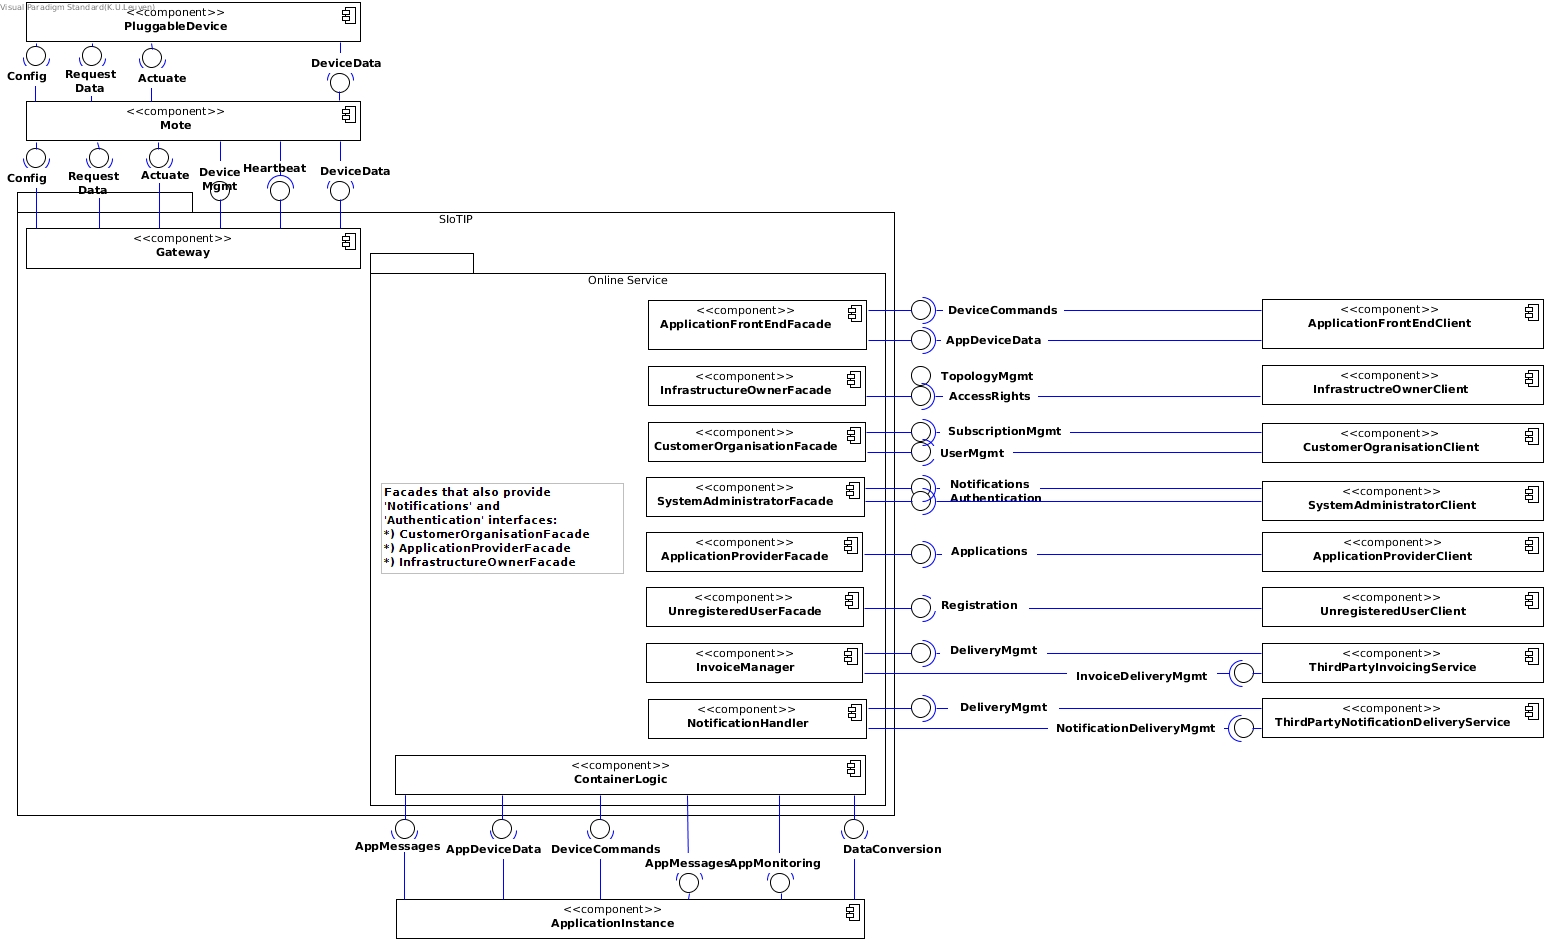
\includegraphics[width=\linewidth]{images/component-CONTEXT}
            \caption{Context diagram for the client-server view.}\label{fig:cc-context}
        \end{figure}

        \vfill
    \end{landscape}

\section{Primary diagram}
    The primary diagram of the client-server view is displayed in figure \ref{fig:cc-primary}. \\

    \todoinline{The primary diagram and accompanying explanation.}

    \begin{landscape}
        \centering
        \vspace*{\fill}

        \begin{figure}[!htp]
            \centering
            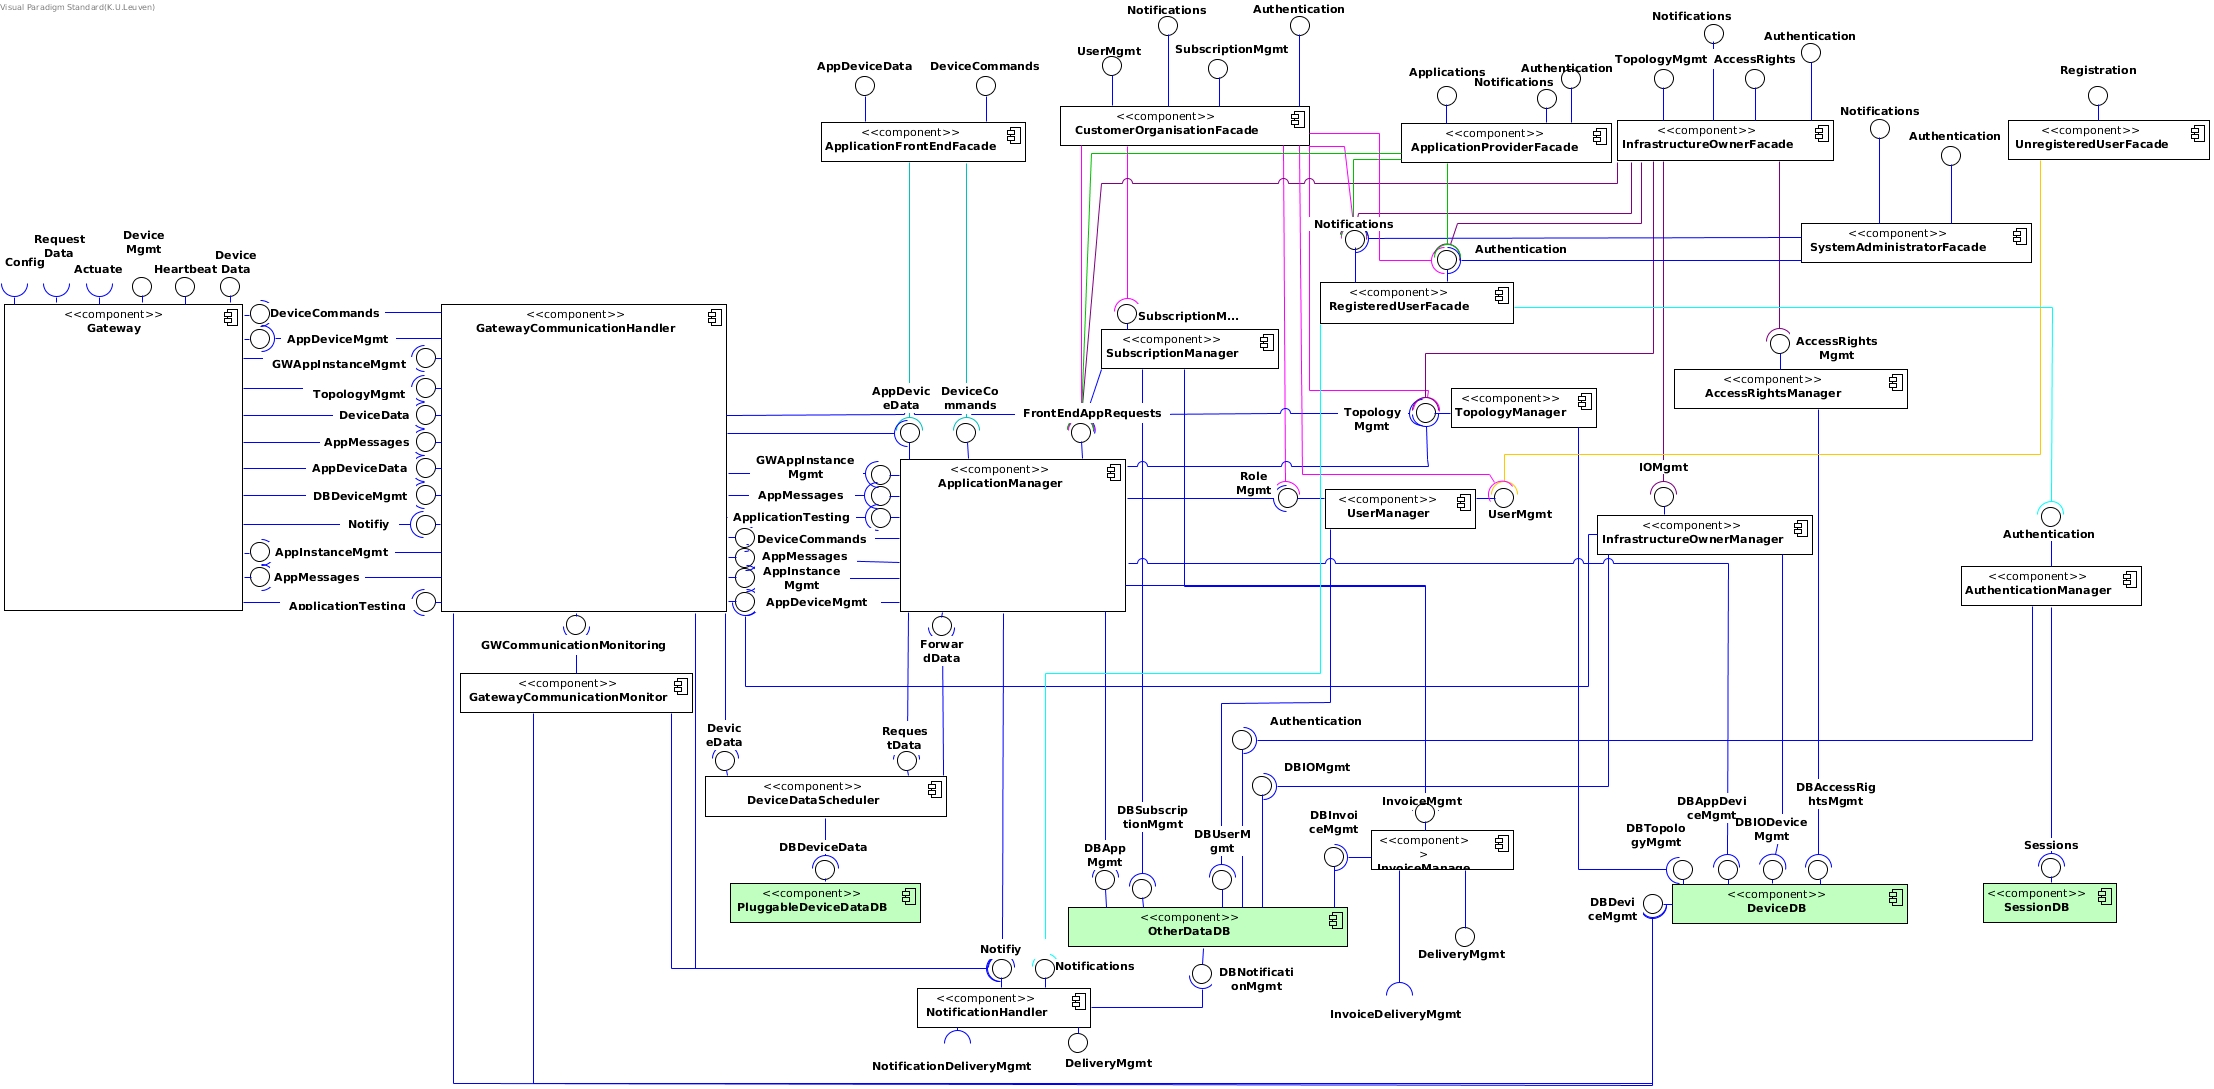
\includegraphics[width=\linewidth]{images/component-PRIMARY}
            \caption{Primary diagram of the client-server view.}\label{fig:cc-primary}
        \end{figure}

        \vfill
    \end{landscape}

    \clearpage

\chapter{Decomposition view (UML Component diagram)}\label{ch:decomposition}
    \minilof
    %\chapter{Decomposition view (UML Component diagram)}\label{ch:decomposition}

% Delete the command below to remove the hints and instructions
\showdecompnotes{}

\begin{figure}[!htp]
	\centering
	%\includegraphics[width=\textwidth]{}
	\missingfigure[figwidth=0.8\textwidth]{Diagram showing decomposition of ComponentX}
	\caption{Decomposition of \texttt{ComponentX}}\label{fig:decomp-componentx}
\end{figure}

\begin{figure}[!htp]
	\centering
	%\includegraphics[width=\textwidth]{}
	\missingfigure[figwidth=0.8\textwidth]{Diagram showing decomposition of ComponentX}
	\caption[Decomposition of \texttt{ComponentY}]{Decomposition of \texttt{ComponentY}.\\
	This caption contains a longer explanation over multiple lines. This additional explanation is not shown in the list of figures.}\label{fig:decomp-componenty}
\end{figure}

    \clearpage
    % \stoplist[decomp]{lof}

\chapter{Deployment view (UML Deployment diagram)}\label{ch:deployment}
    \minilof
    % \chapter{Deployment view (UML Deployment diagram)}\label{ch:deployment}


\begin{landscape}
    \section{Context diagram}
    The context diagram for the deployment view is displayed in figure \ref{fig:depl_context}. \\

    \centering
    \vspace*{\fill}

        \begin{figure}[!htp]
        	\centering
            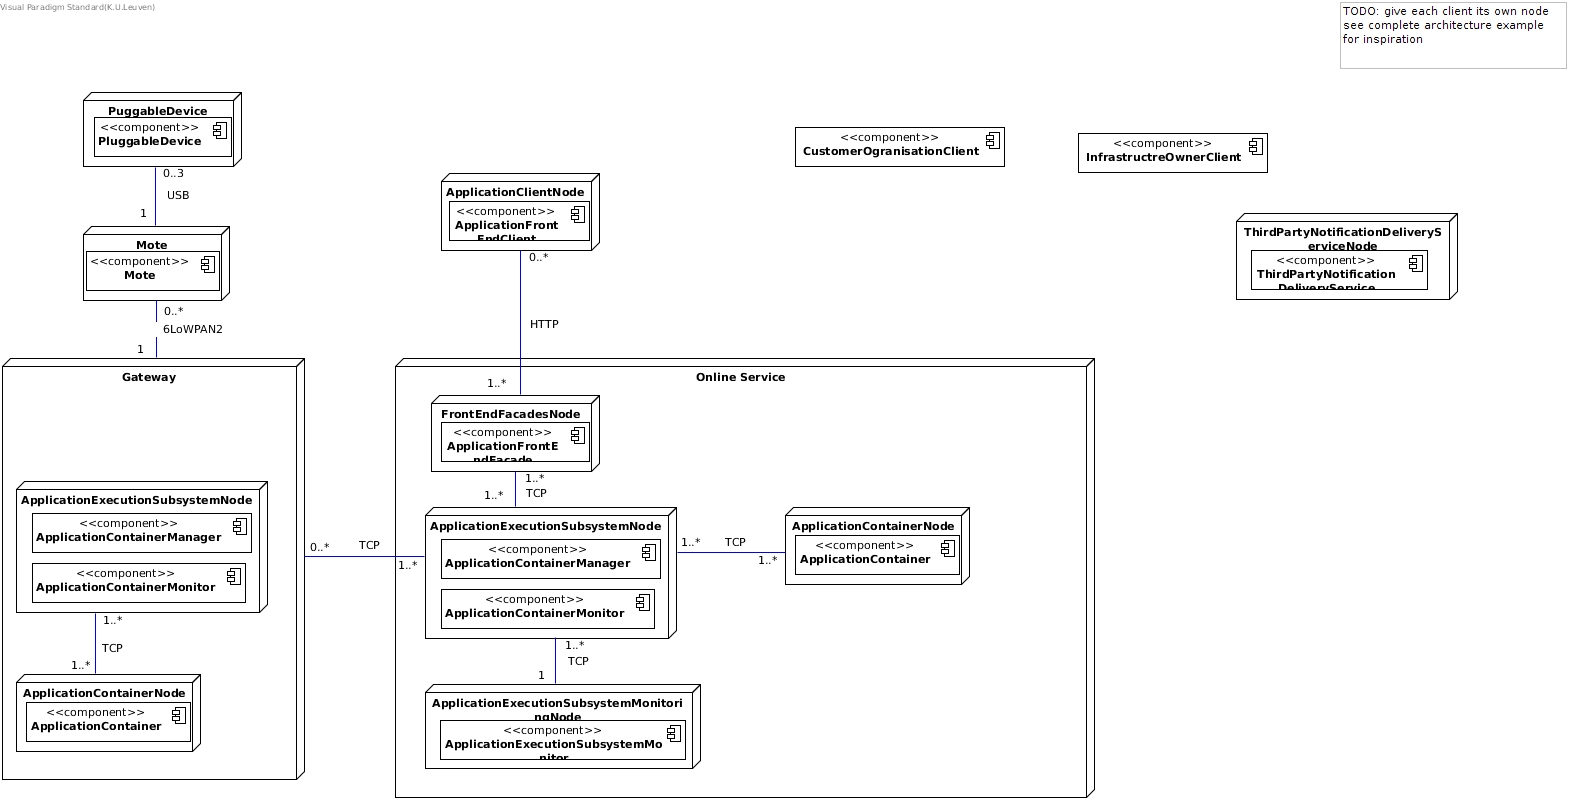
\includegraphics[width=\textwidth]{images/deployment-context}
            \caption{Context diagram for the deployment view.}\label{fig:depl_context}
        \end{figure}

    \vfill
\end{landscape}


\begin{landscape}
    \section{Primary diagram}
    The primary diagram for the deployment view is displayed in figure \ref{fig:depl_primary}.

    \centering
    \vspace*{\fill}

        \begin{figure}[!htp]
        	\centering
            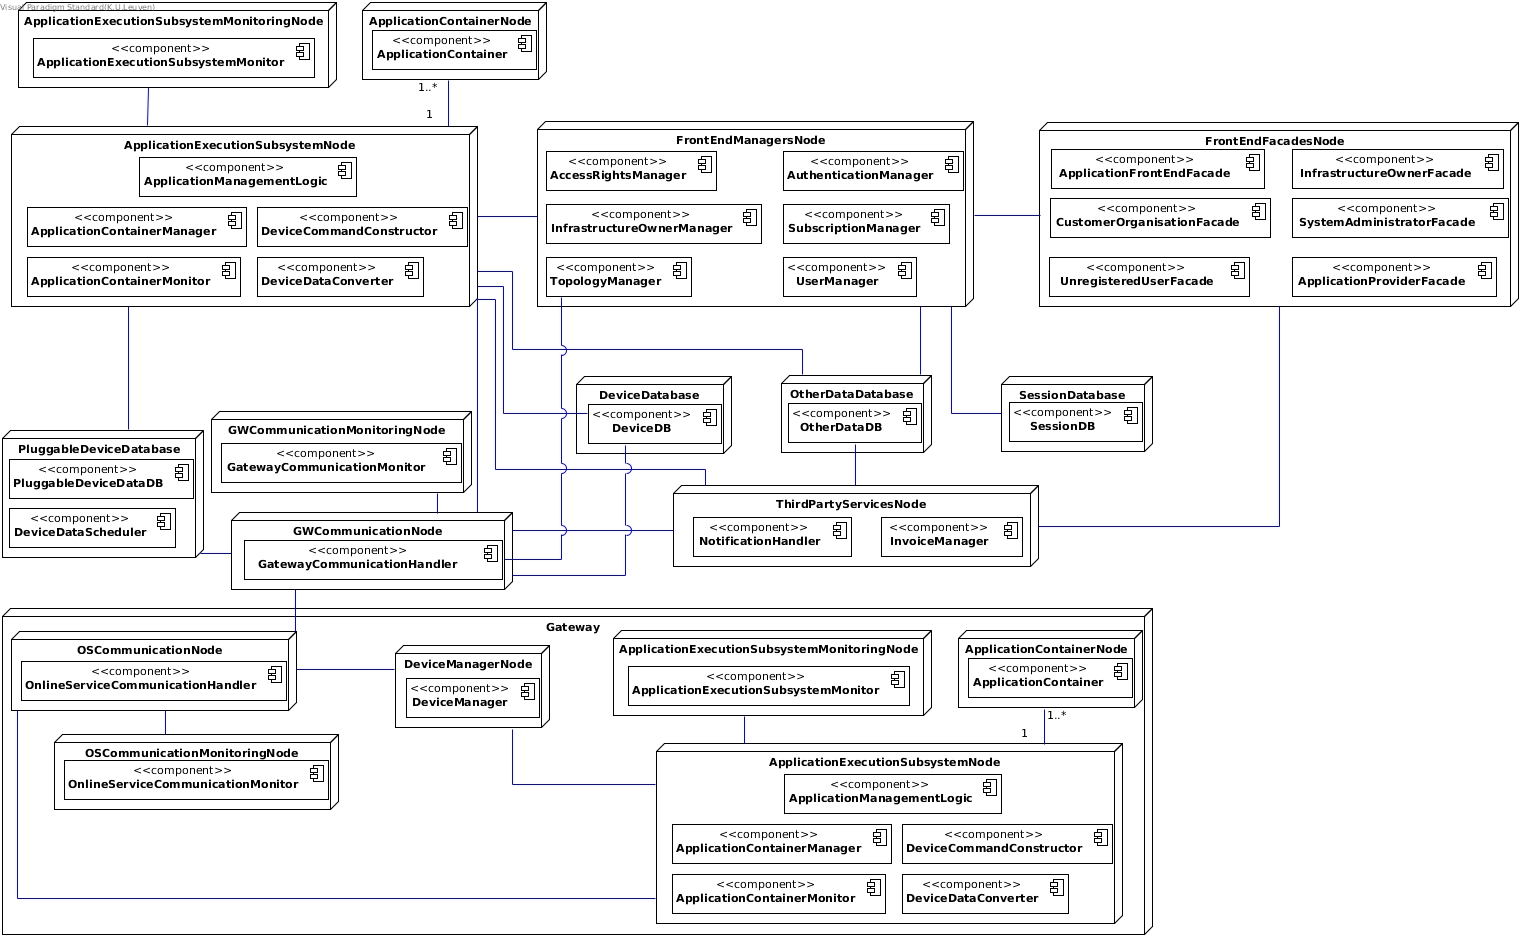
\includegraphics[width=\textwidth]{images/deployment-primary}
        	\caption{Primary diagram for the deployment view.}\label{fig:depl_primary}
        \end{figure}

    \vfill
\end{landscape}

    \clearpage

\chapter{Scenarios}\label{ch:scenarios}
    \minilof
    % \chapter{Scenarios}\label{ch:scenarios}

% Delete the command below to remove the hints and instructions
\showscenariosnotes{}

\todoinline{
	Illustrate how your architecture fulfills the most important data flows. As a rule of thumb, focus on the scenario of the assignment. Describe the scenario in terms of architectural components using UML Sequence diagrams and further explain the most important interactions in text. Illustrating the scenarios serves as a quick validation of the completeness of
	your architecture. If you notice at this point that for some reason, certain functionality or qualities are not addressed sufficiently in your architecture, it suffices to
	document this, together with a rationale of why this is the case according to you. You do not have to further refine you architecture at this point.}


\begin{figure}[!htp]
	\centering
	%\includegraphics[width=\textwidth]{}
	\missingfigure[figwidth=0.8\textwidth]{Sequence diagram scenario 1}
	\caption[Scenario 1]{The system behavior for the first scenario.}\label{fig:seq_scenario1}
\end{figure}


\chapter{Element Catalog and Datatypes}\label{ch:elements-datatypes}
    % \chapter{Element Catalog and Datatypes}\label{ch:elements-datatypes}

% Delete the command below to remove the hints and instructions
\showcatalognotes{}

\section{Element catalog}\label{app:catalog}
    \todoinline{
    List all components and describe their responsibilities and provided
    interfaces.
    Per interface, list all methods using a Java-like syntax and describe their
    effect and exceptions if any.
    List all elements and interfaces alphabetically for ease of navigation.
    }

    \componentItem{ComponentZ}{
    	\begin{itemize}[noitemsep,nolistsep]
    		\item \textbf{Responsibility:} Responsibilities of the component.
    		\item \textbf{Super-component:} The direct super-component, if any.
    		\item \textbf{Sub-components:} the direct sub-components, if any.
    	\end{itemize}
    	\subsubsection*{Provided interfaces}
    	\begin{itemize}[noitemsep,nolistsep]
    		\item InterfaceA
    		\begin{itemize}
    			\item \texttt{returntType1 operation1(ParamType param) throws SomeException}
    			\begin{itemize}
    				\item Effect: Describe the effect of the operation
    			\end{itemize}
    			%
    			\item \texttt{void operation2(ParamType2 param)}
    			\begin{itemize}
    				\item Effect: Describe the effect of the operation
    				\item Exceptions: None
    			\end{itemize}
    		\end{itemize}
    		%
    		\item InterfaceB
    		\begin{itemize}
    			\item \texttt{returntType2 operation3()}
    			\begin{itemize}
    				\item Effect: Describe the effect of the operation
    			\end{itemize}
    		\end{itemize}
    	\end{itemize}
    	}

    \componentItem{ComponentA}{
    	\begin{itemize}[noitemsep,nolistsep]
    		\item \textbf{Responsibility:} Responsibilities of the component.
    		\item \textbf{Super-component:} The direct super-component, if any.
    		\item \textbf{Sub-components:} the direct sub-components, if any.
    	\end{itemize}
    	\subsubsection*{Provided interfaces}
    	\begin{itemize}[noitemsep,nolistsep]
    		\item InterfaceC
    		\begin{itemize}
    			\item \texttt{returntType1 operation1(ParamType param) throws SomeException}
    			\begin{itemize}
    				\item Effect: Describe the effect of the operation
    			\end{itemize}
    			%
    			\item \texttt{void operation2(ParamType2 param)}
    			\begin{itemize}
    				\item Effect: Describe the effect of the operation
    			\end{itemize}
    		\end{itemize}
    		%
    		\item InterfaceD
    		\begin{itemize}[noitemsep,nolistsep]
    			\item \texttt{returntType2 operation3()}
    			\begin{itemize}
    				\item Effect: Describe the effect of the operation
    			\end{itemize}
    		\end{itemize}
    	\end{itemize}
    }

    % This will alphabetically print the list of components.
    \printComponents


\section{Common interfaces}
    \todoinline{If you have any common interfaces used by multiple components you may define them here and refer to them.}

\section{Defined Exceptions}
    \todoinline{Instead of describing the exceptions with each operation, you may define common exceptions here and refer to them from the operation definition.}

\section{Defined data types}\label{app:datatypes}
    \todoinline{
    List and describe all data types defined in your interface specifications. List
    them alphabetically for ease of navigation.
    }

    \begin{itemize}
    	\item \texttt{Paramtype1}: Description of data type.
    	\item \texttt{Paramtype2}: Description of data type.
    	\item \texttt{returnType1}: Description of data type.
    \end{itemize}


\chapter{Attribute-driven design documentation}\label{sec:add}
    \section{Introduction}
        Explain we changed ADD. List of our changes here. \\
        Changed decomposition 1 and 2 compared to part 2a.

    \section{Decomposition 1: SIoTIP System (Av3, UC14, UC15, UC18)}

\subsection{Module to decompose}
    In this run we decompose the \texttt{SIoTIP System}.


\subsection{Selected architectural drivers}
    The non-functional drivers for this decomposition are:
    \begin{itemize}
    	\item \emph{Av3}: Pluggable device or mote failure
    \end{itemize}

    \noindent The related functional drivers are:
    \begin{itemize}
    	\item \emph{UC14}: Send heartbeat (Av3) \\
              This use case checks whether or not motes and pluggable devices
              are still operational.
    	\item \emph{UC15}: Send notification (Av3) \\
              This use case sends a notification to a registered user.
    	\item \emph{UC18}: Check and deactivate applications (Av3) \\
              This use case deactivates any application that requires deactivation,
              because of unavailability of essential pluggable devices
              or unassigned mandatory roles.
    \end{itemize}

    \paragraph{Rationale}
        Av3 was chosen first since it has high priority and it is more relevant to
        the core of the system than the other quality requirements with high
        priority (M1 and U2).
        We believe that handling pluggable device failure/connectivity is
        more important to the whole of the system than M1 and U2, and that
        handling this first would give a stronger starting point for later ADD iterations
        than M1 or U2.


\subsection{Architectural design}\label{sec:architectural-design}
    This section describes what needs to be done to satisfy the requirements for
    this decomposition and how involved problems/obstacles are solved.
    % Detection:
    %     Ping/Echo, Monitor, Heartbeat, Timestamp
    % Resolution:
    %     notifications to 3 stakeholders, degradation/removal from service -> turn off apps

    \paragraph{Av3: Failure detection}
        A SIoTIP gateway can autonomously detect failure of one of its
        connected motes and pluggable devices.
        timers? \\
        heartbeat/timestamp tactic

    \paragraph{Av3: Application deactivation}
        Applications that can no longer operate due to failure of a pluggable
        device or mote should be automatically suspended and re-activated once the failure is resolved.

        Applications need pluggable devices for the proper functioning.
        When the pluggable devices fail, \texttt{the PluggableDeviceManager} sends
        command and \texttt{the ApplicationManager} deactivate one or more applications
        using those devices. Availability and reliability of the shared platform offered to applications is
        important. To reduce the risk of frequent application downtime,
        an application provider can require a redundancy in the available
        pluggable devices. Multiple sensors or actuators for one application can be in one room.
        If one of sensor or actuator failed application just start using
        the other available sensor or actuator in room.

    \paragraph{Av3: Notifications}
        The infrastructure owner should be notified of any persistent pluggable device or mote
        failures. Customer organisations should be notified if one or more of their applications is suspended
        or re-activated. Applications using a failed pluggable device or any device on a failed mote should be
        notified.
        One of the important things for Av3 is notification. In the case
        of failure of sensor, it is mandatory to inform all involved parties
         about the failure to resolve the problem as soon as possible.
        \texttt{The NotificationHandler} notify an infrastructure owner of
        any persistent pluggable device or mote failures. The infrastructure
        owner has to receive the notification in ten seconds in case mote failed or
        in thirty seconds if a pluggable device failed. Notification is also send
        to a customer organisation, when one or more of their application are
        susspended or re-activated. Applications using a failed  pluggable
        device should be also notified via \texttt{The NotificationHandler}.

    \paragraph{Av3: Application redundancy settings}
        Application providers can design their applications such that they explicitly
        require redundancy in the available pluggable devices.

    \subsubsection{Alternatives considered}
        \paragraph{Av3: Alternatives for application deactivation}
            As mentioned above, when some of pluggable devices fail the applation can operate
            normally, because of using the next available sensor. ???? could be?


\subsection{Instantiation and allocation of functionality}
    This section describes the components which instantiate our solutions described
    in the section above and how the components are deployed on physical nodes.

    \paragraph{Decomposition}
        Figure \ref{fig:it1-cc_main} shows the components resulting from the
        decomposition in this run.

        \begin{figure}[!htp]
        	\centering
        	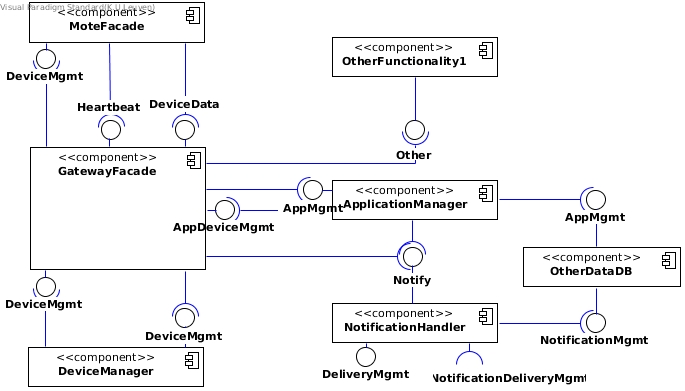
\includegraphics[width=1.00\textwidth]{component-diagram-1}
        	\caption{Component-and-connector diagram of this decomposition.}
            \label{fig:it1-cc_main}
        \end{figure}

        \noindent The responsibilities of the components are as follows:

    \subparagraph{ApplicationManager}
        Responsible for deactivating applications and after this action calls method of
        \texttt{the NotificationHandler} to send notification to a customer organisation.
        When \texttt{the ApplicationManager} detects that application uses failed pluggable devices,
        then the notification is sent to an application.

        set redundancy in the available pluggable devices??
        (Av3) ???? check mandatory user roles

    \subparagraph{Database}
        General database for other data. For instance the Database storages the data
        of notifications (Av3).

    \subparagraph{GatewayFacade}
        Receives heartbeats from pluggable devices and sends heartbeats/device lists.
        \texttt{The GatewayFacade} sends commands to \texttt{the ApplicationManager}
        to shutdown applications, if is it needed. \\

        send notification trigger ???(Av3)\\
        forward data to applications

    \subparagraph{MoteFacade}
        Sends heartbeats from pluggable devices to\texttt{the PluggableDeviceFacade}.

    \subparagraph{NotificationHandler}
        Responsible for send notifications to infrastructure owner, customer organisation
        and applications (Av3). \\
        stored by system \(->\) contact DB? \\
        lookup communication channel \\
        users choose delivery method?

    \subparagraph{PluggableDeviceFacade}
        Sends heartbeats to \texttt{the MoteFacade}.

    \subparagraph{PluggableDeviceManager}
        Checks list of devices and see if there are pluggable devices for applications.
        \texttt{the PluggableDeviceManager} contains application preferences (e.g. amount of sensors required) and
        can send command to deactivate application.
        Send information about new/needed hardware is detected to \texttt{the GatewayFacade}, that sends command to
        reactivate application.
        check redundancy in the available pluggable devices??? is not the same like first sentence???

    % \paragraph{Behaviour}
    % A SEQUENCE DIAGRAM WOULD BE USEFUL FOR
    % UC11: shows how the gateway checks if devices are initialised
    % UC14: shows how applications can get deactivated

    \paragraph{Deployment}
        Figure \ref{fig:it1-depl_main} shows the allocation of components
        to physical nodes.

        \begin{figure}[!htp]
        	\centering
        	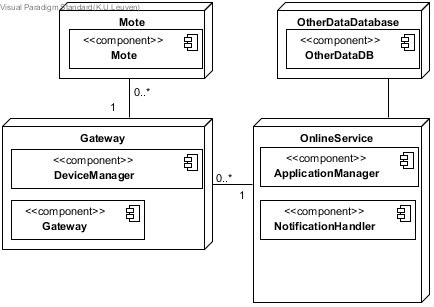
\includegraphics[width=1.00\textwidth]{deployment-diagram-1}
        	\caption{Deployment diagram of this decomposition.}\label{fig:it1-depl_main}
        \end{figure}


\subsection{Interfaces for child modules}\label{add1-interfaces}
    This section describes the interfaces assigned to the components defined
    in the section above. Per interface, we list its methods by means of its
    syntax. The data types used in these interfaces are defined in the following section. \\

    \noindent Each method shows which (part of a) quality attribute or use case caused
    a need for the method. However, this does not mean that a method is
    only to be used to satisfy that quality  attribute or use case, it could
    be used for other causes not yet mentioned here.

    \subsubsection{ApplicationManager}
        \begin{itemize}
            \item ForwardData
            \begin{itemize}
                \item \texttt{void sendData(PluggableDeviceData data)}
                \begin{itemize}
                    \item Effect: Send pluggable device data to an application that wants to use it
                    \item Created for:
                \end{itemize}
            \end{itemize}

            \item AppMgmt
            \begin{itemize}
                \item \texttt{void deactivateApplicationInstance(int applicationInstanceID)}
                \begin{itemize}
                    \item Effect: Deactivates a running instance of an application.
                    \item Created for:
                \end{itemize}
                \item \texttt{void activateApplicationInstance(int applicationInstanceID)}
                \begin{itemize}
                    \item Effect: Activates a new instance of an application.
                    \item Created for:
                \end{itemize}
            \end{itemize}
        \end{itemize}

    \subsubsection{Database}
        \begin{itemize}
            \item NotificationMgmt
            \begin{itemize}
                \item \texttt{int storeNotification(NotificationData data)}
                \begin{itemize}
                    \item Effect: Stores a new notification entry in the database. Returns the id of the new notification.
                    \item Created for:
                \end{itemize}
                \item \texttt{void updateNotification(NotificationData data)}
                \begin{itemize}
                    \item Effect: Updates an existing notification (e.g. change status to "sent").
                    \item Created for:
                \end{itemize}
                \item \texttt{int lookupNotificationChannelForUser(int userID)}
                \begin{itemize}
                    \item Effect: Returns the type of communication channel a user prefers.
                                  Different communication channels are mapped to integers.
                    \item Created for:
                \end{itemize}
            \end{itemize}

            \item AppDataMgmt
            \begin{itemize}
                \item \texttt{void updateApplication(ApplicationData data)}
                \begin{itemize}
                    \item Effect: Updates an application in the database (e.g. change state to 'inactive').
                    \item Created for:
                \end{itemize}
                \item \texttt{void updateSubscription(SubscriptionData data)}
                \begin{itemize}
                    \item Effect: Updates a subscription in the database (e.g. change state to 'disabled').
                    \item Created for:
                \end{itemize}
            \end{itemize}
        \end{itemize}

    \subsubsection{GatewayFacade}
        \begin{itemize}
            \item MoteDataMgmt
            \begin{itemize}
                \item \texttt{void sendHeartbeat(int moteID, List<PluggableDeviceInfo> devices)}
                \begin{itemize}
                    \item Effect: Sends a heartbeat to a certain gateway with information about operational devices.
                    \item Created for:
                \end{itemize}
            \end{itemize}

            \item DeviceMgmt
            \begin{itemize}
                \item \texttt{List<DeviceInfo> getConnectedDevices()}
                \begin{itemize}
                    \item Effect: Describe the effect of calling this operation.
                    \item Created for:
                \end{itemize}
                \item \texttt{void timerExpired(int deviceID)}
                \begin{itemize}
                    \item Effect: Lets the gateway know that a timer for pluggable device or mote has expired.
                                  This will generate a notification for an infrastructure owner.
                    \item Created for:
                \end{itemize}
                \item \texttt{void deactivateApplicationInstance(int applicationInstanceID)}
                \begin{itemize}
                    \item Effect: Deactivates a certain application. This could happen when
                                  mandatory pluggable devices for the application are missing.
                    \item Created for:
                \end{itemize}
                \item \texttt{void reactivateApplicationInstance(int applicationInstanceID)}
                \begin{itemize}
                    \item Effect: Reactivate an application instance. This could happen
                                  automatically after a broken sensor has been replaced.
                    \item Created for:
                \end{itemize}
            \end{itemize}

            \item AppDeviceMgmt
            \begin{itemize}
                \item \texttt{bool areEssentialDevicesOperational(int applicationID)}
                \begin{itemize}
                    \item Effect: Returns true if all essential devices for the application
                                  with id "applicationID" are operational.
                    \item Created for:
                \end{itemize}
            \end{itemize}
        \end{itemize}

    \subsubsection{MoteFacade}
        \begin{itemize}
            \item PluggableDeviceDataMgmt
            \begin{itemize}
                \item \texttt{List<DeviceInfo> getConnectedDevices()}
                \begin{itemize}
                    \item Effect: Returns a list of information about devices that are connected to the mote.
                    \item Created for:
                \end{itemize}
            \end{itemize}
        \end{itemize}

    \subsubsection{NotificationHandler}
        \begin{itemize}
            \item Notify
            \begin{itemize}
                \item \texttt{void notify(int userID, String message)}
                \begin{itemize}
                    \item Effect: Describe the effect of calling this operation.
                    \item Created for:
                \end{itemize}
            \end{itemize}

            \item DeliveryMgmt
            \begin{itemize}
                \item \texttt{void sendAcknowledgement(int notificationID)}
                \begin{itemize}
                    \item Effect: Sends an acknowledgement to the system for a certain notification.
                    \item Created for:
                \end{itemize}
            \end{itemize}
        \end{itemize}

    \subsubsection{External notification delivery serivce}
        \begin{itemize}
            \item NotificationDeliveryMgmt
            \begin{itemize}
                \item \texttt{void notify(JSONObject data)}
                \begin{itemize}
                    \item Effect: Deliver a notification to an end user using a specific delivery service.
                    \item Created for:
                \end{itemize}
            \end{itemize}
        \end{itemize}

    \subsubsection{PluggableDeviceManager}
        \begin{itemize}
        	\item DeviceListMgmt
        	\begin{itemize}
        		\item \texttt{void sendHeartbeat(int moteID, List<PluggableDeviceInfo> devices)}
        		\begin{itemize}
        			\item Effect: Send a heartbeat from a mote to check/update timers for operational devices.
        			\item Created for:
        		\end{itemize}
        		\item \texttt{bool areEssentialDevicesOperational(int applicationID)}
        		\begin{itemize}
        			\item Effect: Returns true if all essential devices for the application
                                  with id "applicationID" are operational.
        			\item Created for:
        		\end{itemize}
        	\end{itemize}
        \end{itemize}


\subsection{Data type definitions}
    This section defines the data types used in the interface descriptions above.

    \paragraph{PluggableDeviceData}
              contains data from a pluggable device at a certain point in time
              (value, type, date) (e.g. a sensor reading, an actuator status)
    \paragraph{PluggableDeviceSettings}
              contains settings for a pluggable device (power status,
              data update rate, ...)
    \paragraph{PluggableDeviceInfo}
              contains information about a pluggable device (device id,
              power status, data update rate, ...)
    \paragraph{NotificationData}
              contains data about a notification (message text, recipient,
              communication channel, date, status, source, ...).
    \paragraph{ApplicationData}
              contains data about an application instance (instance id, running status, ...)
    \paragraph{SubscriptionData}
              contains data about a subscription (subscription id, subscription status,
              subscription period, ...).


\subsection{Verify and refine}
    \noindent The selected architectural drivers have been handled completely
    in this decomposition.
    This section describes per component which (parts of) the remaining
    requirements it is responsible for. If requirements are split in
    multiple parts, this is indicated by the addition of a letter
    (or number, depending on the structure of the requirement) after their title.

    \paragraph{ApplicationManager}
        \begin{itemize}
            \item \emph{Av2}: Application failure \\
                   Prevention: a, b \\
                   Detection: a, b, c \\
                   Resolution: a, b, c
           \item \emph{P1}: Large number of users: c
           \item \emph{M1}: Integrate new sensor or actuator manufacturer: 1.c, 2.a
           \item \emph{M2}: Big data analytics on pluggable data and/or application usage data: d, e
           \item \emph{U1}: Application updates: a, b, c, d
           \item \emph{U2}: Easy Installation: e
           \item \emph{UC12}: Perform actuation command
           \item \emph{UC17}: Activate an application: 3, 4
        \end{itemize}

    \paragraph{Database}
        \begin{itemize}
          	\item None
        \end{itemize}

    \paragraph{GatewayFacade}
        \begin{itemize}
            \item \emph{Av1}: Communication between SIoTIP gateway and Online Service \\
                               Resolution: b, c, d
            \item \emph{M1}: Integrate new sensor or actuator manufacturer: 1.a, 2.b
            \item \emph{U2}: Easy Installation: a, c, d
            \item \emph{UC11}: Send pluggable device data: 1
        \end{itemize}

    \paragraph{MoteFacade}
        \begin{itemize}
            \item \emph{M1}: Integrate new sensor or actuator manufacturer: 1.a, 2.b
            \item \emph{U2}: Easy Installation: b, c, d
            \item \emph{UC04}: Install mote: 1, 2
            \item \emph{UC05}: Uninstall mote: 1
            \item \emph{UC06}: Insert a pluggable device into a mote: 2
            \item \emph{UC07}: Remove a pluggable device from its mote: 2
            \item \emph{UC11}: Send pluggable device data: 1
        \end{itemize}

    \paragraph{NotificationHandler}
        \begin{itemize}
            \item \emph{UC16}: Consult notification message: 5
            \item \emph{UC17}: Activate an application: 5, 6
        \end{itemize}

    \paragraph{OtherFunctionality1}
        \begin{itemize}
            \item \emph{Av1}: Communication between SIoTIP gateway and Online Service \\
                               Detection: a, b, c, d
                               Resolution: a
           	\item \emph{P1}: Large number of users: a
            \item \emph{P2}: Requests to the pluggable data database
            \item \emph{M1}: Integrate new sensor or actuator manufacturer: 1.d
            \item \emph{M2}: Big data analytics on pluggable data and/or application usage data: a
            \item \emph{U2}: Easy Installation: e
            \item \emph{UC01}: Register a customer organisation
            \item \emph{UC02}: Register an end-user
            \item \emph{UC03}: Unregister an end user
            \item \emph{UC04}: Install mote: 3
            \item \emph{UC05}: Uninstall mote: 2.b
            \item \emph{UC06}: Insert a pluggable device into a mote: 3: topology part; alternative 3a.1.b
            \item \emph{UC07}: Remove a pluggable device from its mote: 3.b
            \item \emph{UC08}: Initialise a pluggable device: 1, 2, 4
            \item \emph{UC09}: Configure pluggable device access rights
            \item \emph{UC10}: Consult and configure the topology
            \item \emph{UC11}: Send pluggable device data: 3
            \item \emph{UC13}: Configure pluggable device
            \item \emph{UC16}: Consult notification message: 1, 2, 3, 4
            \item \emph{UC17}: Activate an application: 1, 2
            \item \emph{UC19}: Subscribe to application
            \item \emph{UC20}: Unsubscribe from application
            \item \emph{UC21}: Send invoice
            \item \emph{UC22}: Upload an application
            \item \emph{UC23}: Consult application statistics
            \item \emph{UC24}: Consult historical data
            \item \emph{UC25}: Access topology and available devices
            \item \emph{UC26}: Send application command or message to external front-end
            \item \emph{UC27}: Receive application command or message to external front-end
            \item \emph{UC28}: Log in
            \item \emph{UC29}: Log out
        \end{itemize}

    \paragraph{PluggableDeviceFacade}
        \begin{itemize}
        	\item \emph{U2}: Easy Installation: d
        \end{itemize}

    \paragraph{PluggableDeviceManager}
        \begin{itemize}
            \item \emph{U2}: Easy Installation: c, d
            \item \emph{UC04}: Install mote: 4
            \item \emph{UC05}: Uninstall mote: 2
            \item \emph{UC06}: Insert a pluggable device into a mote: 3: uninitialised part; alternative 3a.1 3a.2 3a.4; 4
            \item \emph{UC07}: Remove a pluggable device from its mote: 3.a, 3.c
            \item \emph{UC08}: Initialise a pluggable device: 3
            \item \emph{UC11}: Send pluggable device data: 2, 3a
        \end{itemize}

    \newpage
    \section{Decomposition 2: OtherFunctionality1 (M1, P2, UC11)}

\subsection{Module to decompose}
    In this run we decompose OtherFunctionality1.


\subsection{Selected architectural drivers}
    The non-functional drivers for this decomposition are:
    \begin{itemize}
    	\item \emph{M1}: Integrate new sensor or actuator manufacturer
        \item \emph{P2}: Requests to the pluggable data database
    \end{itemize}

    \noindent The related functional drivers are:
    \begin{itemize}
        \item \emph{UC11}: Send pluggable device data (P2) \\
              This use case stores pluggable device data in the pluggable device data storage.
              This could be a sensor reading or an actuator status.
    \end{itemize}

    \paragraph{Rationale}
    We chose M1 as it was one of the remaining quality attributes with high priority.
    M1's focus on easily introducing new types of devices to the system is very important
    because of the fast growing market for IoT and development of applications for IoT.
    Thus, we want to handle this quality attribute before U2 (the other remaining
    attribute with high priority), as we presume that customer organisations
    are more interested in using new devices than the effort it takes for
    infrastructure owners to install the devices. \\
    We also chose P2 because it is strongly related to M1; the whole data flow from
    devices to storage/applications needs to exist before modifications can even be made.
    This combination of M1 and P2 would force us to handle processing and
    storage of data while making the involved components as simple as possible to modify.


\subsection{Architectural design}
    This section describes what needs to be done to satisfy the requirements for
    this decomposition and how involved problems/obstacles are solved.
    % Tactics:
    %     Limit event response? reply within response measure deadlines
    %     Prioritize events
    %     Introduce concurrency
    %     Schedule resources

    % Tactics M1:
    %     reduce size of modules: split module

    \paragraph{M1: Handling new types of pluggable devices}
        The new types of sensor or actuator data should be transmitted, processed and stored,
        and should be made available to applications. The infrastructure managers must be able to initialize the new type of pluggable device
        (UC8 : Initialise a pluggable device), configure access rights for these devices (UC9 : Con-
        figure pluggable device access rights), and view detailed information about the new type
        of pluggable device (UC10 : Consult and configure the topology).

        The developers have to make changes to: component1, component2, datatype X.
        The new type of sensor needs to be able to be initialised so that it can send data.
        Thus, the PluggableDeviceFacade code that initialises devices should be updated for
        each new type of sensor. The PluggableDeviceData datatype should be updated to
        represent the new type of data. In this case, the new type will have to be added
        to the database that contains all different types of sensor data.

    \paragraph{M1: Data conversions}
        The pluggable data processing subsystem should be extended with relevant data conver-
        sions, e.g. converting temperature in degrees Fahrenheit to degrees Celsius.
        \texttt{The PluggableDeviceDataConverter} is resposible for converting data
        in system, for instance converting temperature in degrees Fahrenheit
        to degrees Celsius. System has to work with relevant data,
        otherwise problem may arise.

    \paragraph{M1: Usage of new data by applications}
        The available applications can be updated to use any new pluggable devices.
        This is possible through the RequestData interface provided by PluggableDeviceDataScheduler.
        The application manager can get device data from the PluggableDeviceDB and return this
        data to applications in the PluggableDeviceData datatype. This datatype can easily be
        updated for new types of pluggable devices.

    \paragraph{M1: Configuration of new device by infrastructure owners}
        Initialisation: IO triggers the initialise() method which has been
        updated for the new pluggable device -> OK\\
        Configure access rights: has absolutely fucking nothing to do with the
        new sensor type -> OK \\
        Consult and configure topology: same as configure access rights

    \paragraph{P2: Scheduling}
        - In normal mode, the database processes incoming requests in a first-in-first-out order.
        - If the system fails to comply to the deadlines specified below, it goes in overload mode: requests
            are handled in the order that returns the system to normal mode the fastest, taking into
            account:
            ∗ the nature of the requests: storing new pluggable data (UC11 : Send pluggable device
            data) has priority over specific lookup queries (e.g. retrieving most recent measurement
            for a few sensors), which in turn have priority over broad queries (e.g. retrieving all sensor
            data for the last month).
            ∗ the priority of an application: requests from applications marked as critical by their sub-
            scribers are processed before non-critical applications.
        - Also a mechanism should be in place to avoid starvation of any type of request.

        dynamic priority scheduling \\
        tactics: schedule resource, prioritize events, also limit event response?\\
        starvation avoidance

    \paragraph{P2: Pluggable data separation}
        The processing of (large amounts of) requests concerning pluggable data has no impact on
        requests concerning other data, e.g. available applications.

        "pluggable data has no impact on other data"
        two databases

    \subsubsection{Alternatives considered}
        \paragraph{P2: Alternatives for Scheduling}
        In overload mode, a high priority process will run before a low priority process. 
        It can cuase that the low priority process will never be scheduled.
        Our scheduling algorithms will contain code to guarantee that all processes will 
        receive a minimum amount of each important resource (e.g. CPU time) in order to avoid starvation.


\subsection{Instantiation and allocation of functionality}
    This section describes the new components which instantiate our solutions described
    in the section above and how components are deployed on physical nodes. \\
    Unless stated otherwise the responsibilities assigned in the first decomposition are unchanged.

    \paragraph{Decomposition}
        Figure \ref{fig:it2-cc_main} shows the components resulting from the
        decomposition in this run.

        \begin{figure}[!h]
        	\centering
            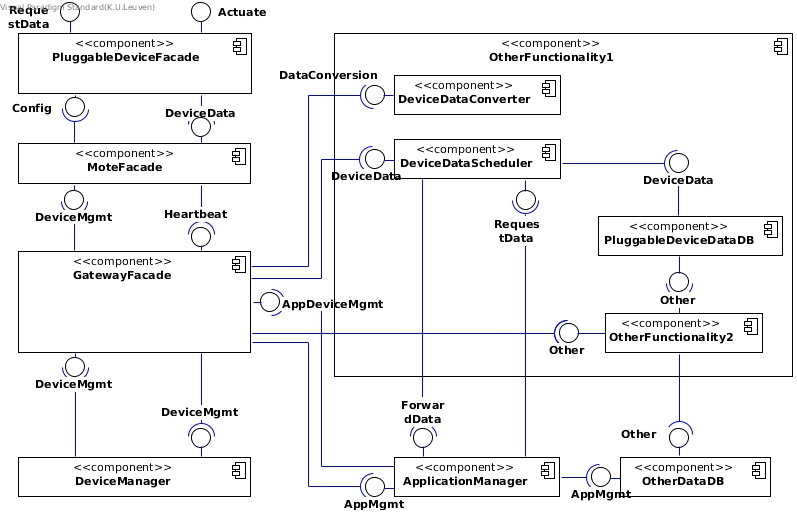
\includegraphics[width=1\textwidth]{component-diagram-2}
        	\caption{Component-and-connector diagram of this decomposition.}
            \label{fig:it2-cc_main}
        \end{figure}

        \noindent The responsibilities of the components are as follows:

    \subparagraph{PluggableDeviceDB}
        stores data related to pluggable devices. In \texttt{the PluggableDeviceDB}
        is stored basic information about devices.

    \subparagraph{PluggableDeviceDataScheduler}
        \texttt{the PluggableDeviceDB} receives a large amount of parallel request
        and it is neccesary to handle with that.
        \texttt{The PluggableDeviceDataScheduler} is resposnsible for scheduling jobs
        that interact with database. Jobs are processed in a first-in-first-out order normaly.
        In case te overload mode is detected, jobs are proccesed in  the  order
        that  returns  the  system. In case the data has to be saved,
        \texttt{The PluggableDeviceDataScheduler} call method for saving the data, that
         \texttt{the PluggableDeviceDB} provides.

    \subparagraph{PluggableDeviceDataConverter}
       is component for conversions of new type of data of new type of device (M1).
       For instance converting temperature is very useful in the system.

    % \paragraph{Behaviour}
        % A SEQUENCE DIAGRAM WOULD BE USEFUL FOR
        % UC11: shows how the gateway checks if devices are initialised
        % UC14: shows how applications can get deactivated

    \paragraph{Deployment}
        Figure \ref{fig:it2-depl_main} shows the allocation of components
        to physical nodes.

        \begin{figure}[!h]
        	\centering
        	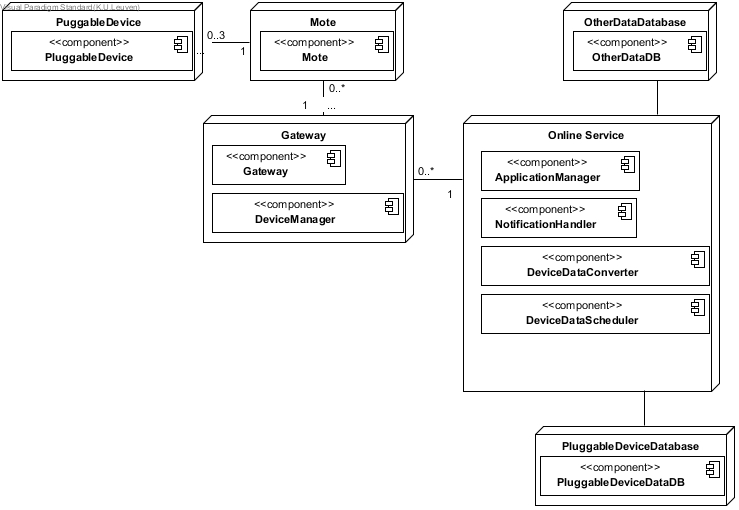
\includegraphics[width=1\textwidth]{deployment-diagram-2}
        	\caption{Deployment diagram of this decomposition.
        	}\label{fig:it2-depl_main}
        \end{figure}


\subsection{Interfaces for child modules}\label{add2-interfaces}
    This section describes the interfaces assigned to the components defined
    in the section above. Per interface, we list its methods by means of its
    syntax. The data types used in these interfaces are defined in the following section. \\

    \noindent Each method shows which (part of a) quality attribute or use case caused
    a need for the method. However, this does not mean that a method is
    only to be used to satisfy that quality  attribute or use case, it could
    be used for other causes not yet mentioned here.

    \noindent The interfaces and methods defined here are to be seen as an
    extension of the interfaces defined in previous sections, unless
    explicitly stated otherwise.

    \subsubsection{GatewayFacade}
        \begin{itemize}
            \item MoteDataMgmt, last defined in section \ref{add1-interfaces}
            \begin{itemize}
                \item \texttt{void sendData(PluggableDeviceData data)}
                \begin{itemize}
                    \item Effect: Sends pluggable device data to the connected mote.
                    \item Created for:
                \end{itemize}
            \end{itemize}

            \item DeviceMgmt, last defined in section \ref{add1-interfaces}
            \begin{itemize}
                \item \texttt{void initialiseDevice(int deviceID, PluggableDeviceSettings settings)}
                \begin{itemize}
                    \item Effect: Initialises a pluggable device for use with the system.
                    \item Created for:
                \end{itemize}
            \end{itemize}

            \item AppDeviceMgmt, last defined in section \ref{add1-interfaces}
            \begin{itemize}
                \item \texttt{void configurePluggableDevice(int deviceID, PluggableDeviceSettings settings)}
                \begin{itemize}
                    \item For: Use case 11 step 3.b
                    \item Effect: Causes certain settings to be set on a pluggable
                          device that the gateway is connected to.
                    \item Created for:
                \end{itemize}
            \end{itemize}
        \end{itemize}

    \subsubsection{MoteFacade}
        \begin{itemize}
            \item PluggableDeviceDataMgmt, last defined in section \ref{add1-interfaces}
            \begin{itemize}
                \item \texttt{void sendData(PluggableDeviceData data)}
                \begin{itemize}
                    \item Effect: Sends pluggable device data to the connected mote.
                    \item Created for:
                \end{itemize}
            \end{itemize}

            \item PluggableDeviceMgmt
            \begin{itemize}
                \item \texttt{void initialise(int deviceID, PluggableDeviceSettings settings)}
                \begin{itemize}
                    \item Effect: Initialises a connected pluggable device according to some settings
                    \item Created for:
                \end{itemize}
            \end{itemize}
        \end{itemize}

    \subsubsection{PluggableDeviceFacade}
        \begin{itemize}
        	\item PluggableDeviceMgmt
        	\begin{itemize}
                \item \texttt{void initialise(PluggableDeviceSettings settings)}
                \begin{itemize}
                    \item Effect: Initialises the pluggable device according to some settings
                    \item Created for:
                \end{itemize}
        	\end{itemize}
        \end{itemize}

    \subsubsection{PluggableDeviceManager}
        \begin{itemize}
        	\item DeviceListMgmt, last defined in section \ref{add1-interfaces}
        	\begin{itemize}
        		\item \texttt{bool isDeviceInitialised(int deviceID)}
        		\begin{itemize}
        			\item Effect: Returns true if the device with id "deviceID" has been initialized.
        			\item Created for:
        		\end{itemize}
        	\end{itemize}
        \end{itemize}

    \subsubsection{PluggableDeviceDataScheduler}
        \begin{itemize}
            \item RequestData
            \begin{itemize}
                \item \texttt{List<PluggableDeviceData> requestData(int applicationID, int deviceID, DateTime from, DateTime to)}
                \begin{itemize}
                    \item Effect: Request data from a specific device in a certain time period
                    \item Created for:
                \end{itemize}
            \end{itemize}

            \item PluggableDeviceDataMgmt
            \begin{itemize}
                \item \texttt{void sendData(PluggableDeviceData data)}
                \begin{itemize}
                    \item Effect: Sends pluggable device data to the scheduler to be processed.
                    \item Created for:
                \end{itemize}
            \end{itemize}
        \end{itemize}

    \subsubsection{PluggableDeviceDB}
        \begin{itemize}
            \item PluggableDeviceDataMgmt
            \begin{itemize}
                \item \texttt{void sendData(PluggableDeviceData data)}
                \begin{itemize}
                    \item Effect: Sends pluggable device data to the DB to be stored.
                    \item Created for:
                \end{itemize}
                \item \texttt{List<PluggableDeviceData> getData(int deviceID, DateTime from, DateTime to)}
                \begin{itemize}
                    \item Effect: Returns data from a specific device in a certain time period.
                    \item Created for:
                \end{itemize}
                \item \texttt{List<int> getApplicationsForDevice(int deviceID)}
                \begin{itemize}
                    \item Effect: Returns a list of applications that can use the device with id "deviceID."
                    \item Created for:
                \end{itemize}
            \end{itemize}
        \end{itemize}


\subsection{Data type definitions}
    This section defines new data types that are used in the interface descriptions above.

    \paragraph{DateTime} Represents an instant in time, typically expressed as a date and time of day.


\subsection{Verify and refine}
    \noindent The selected architectural drivers have been handled completely
    in this decomposition.
    This section describes per component which (parts of) the remaining
    requirements it is responsible for. If requirements are split in
    multiple parts, this is indicated by the addition of a letter
    (or number, depending on the structure of the requirement) after their title.

    \paragraph{ApplicationManager}
        \begin{itemize}
            \item \emph{Av2}: Application failure \\
                   Prevention: a, b \\
                   Detection: a, b, c \\
                   Resolution: a, b, c
           \item \emph{P1}: Large number of users: c
           \item \emph{M2}: Big data analytics on pluggable data and/or application usage data: d, e
           \item \emph{U1}: Application updates: a, b, c, d
           \item \emph{U2}: Easy Installation: e
           \item \emph{UC12}: Perform actuation command
           \item \emph{UC17}: Activate an application: 3, 4
        \end{itemize}

    \paragraph{Database}
        \begin{itemize}
          	\item None
        \end{itemize}

    \paragraph{GatewayFacade}
        \begin{itemize}
            \item \emph{Av1}: Communication between SIoTIP gateway and Online Service \\
                               Resolution: b, c, d
            \item \emph{U2}: Easy Installation: a, c, d
        \end{itemize}

    \paragraph{MoteFacade}
        \begin{itemize}
            \item \emph{U2}: Easy Installation: b, c, d
            \item \emph{UC04}: Install mote: 1, 2
            \item \emph{UC05}: Uninstall mote: 1
            \item \emph{UC06}: Insert a pluggable device into a mote: 2
            \item \emph{UC07}: Remove a pluggable device from its mote: 2
        \end{itemize}

    \paragraph{NotificationHandler}
        \begin{itemize}
            \item \emph{UC16}: Consult notification message: 5
            \item \emph{UC17}: Activate an application: 5, 6
        \end{itemize}

    \paragraph{OtherFunctionality2}
        \begin{itemize}
            \item \emph{Av1}: Communication between SIoTIP gateway and Online Service \\
                               Detection: a, b, c, d
                               Resolution: a
           	\item \emph{P1}: Large number of users: a
            \item \emph{M2}: Big data analytics on pluggable data and/or application usage data: a
            \item \emph{U2}: Easy Installation: e
            \item \emph{UC01}: Register a customer organisation
            \item \emph{UC02}: Register an end-user
            \item \emph{UC03}: Unregister an end user
            \item \emph{UC04}: Install mote: 3
            \item \emph{UC05}: Uninstall mote: 2.b
            \item \emph{UC06}: Insert a pluggable device into a mote: 3: topology part; alternative 3a.1.b
            \item \emph{UC07}: Remove a pluggable device from its mote: 3.b
            \item \emph{UC08}: Initialise a pluggable device: 1, 2, 4
            \item \emph{UC09}: Configure pluggable device access rights
            \item \emph{UC10}: Consult and configure the topology
            \item \emph{UC13}: Configure pluggable device
            \item \emph{UC16}: Consult notification message: 1, 2, 3, 4
            \item \emph{UC17}: Activate an application: 1, 2
            \item \emph{UC19}: Subscribe to application
            \item \emph{UC20}: Unsubscribe from application
            \item \emph{UC21}: Send invoice
            \item \emph{UC22}: Upload an application
            \item \emph{UC23}: Consult application statistics
            \item \emph{UC24}: Consult historical data
            \item \emph{UC25}: Access topology and available devices
            \item \emph{UC26}: Send application command or message to external front-end
            \item \emph{UC27}: Receive application command or message to external front-end
            \item \emph{UC28}: Log in
            \item \emph{UC29}: Log out
        \end{itemize}

    \paragraph{PluggableDeviceDB}
        \begin{itemize}
            \item \emph{M2}: Big data analytics on pluggable data and/or application usage data: b
        \end{itemize}

    \paragraph{PluggableDeviceFacade}
        \begin{itemize}
        	\item \emph{U2}: Easy Installation: d
        \end{itemize}

    \paragraph{PluggableDeviceManager}
        \begin{itemize}
            \item \emph{U2}: Easy Installation: c, d
            \item \emph{UC04}: Install mote: 4
            \item \emph{UC05}: Uninstall mote: 2
            \item \emph{UC06}: Insert a pluggable device into a mote: 3: uninitialised part; alternative 3a.1 3a.2 3a.4; 4
            \item \emph{UC07}: Remove a pluggable device from its mote: 3.a, 3.c
            \item \emph{UC08}: Initialise a pluggable device: 3,
        \end{itemize}

    \paragraph{PluggableDeviceDataScheduler}
        \begin{itemize}
            \item \emph{P1}: Large number of users: b
            \item \emph{M2}: Big data analytics on pluggable data and/or application usage data: b, c
        \end{itemize}

    \newpage
    \section{Decomposition 3: U2, UC4, UC6, UC9, UC10, UC17, UC19.7-11}

\subsection{Elements/Subsystem to decompose/expand}
    In this run we decompose/expand ...


\subsection{Selected architectural drivers}
    The non-functional drivers for this decomposition are:
    \begin{itemize}
    	\item \emph{U2}: Easy installation
    \end{itemize}

    The related functional drivers are:
    \begin{itemize}
        \item \emph{UC4}: Install mote \\
              Short description
        \item \emph{UC6}: Insert a pluggable device into a mote \\
              Short description
        \item \emph{UC9}: Configure pluggable device access rights \\
              Short description
        \item \emph{UC10}: Consult and configure topology \\
              Short description
        \item \emph{UC17}: Activate an application \\
              Short description
        \item \emph{UC19}: Subscribe to application \\
              Short description
    \end{itemize}


\subsection{Architectural design}
    This section describes what needs to be done to satisfy the requirements for
    this decomposition and how involved problems/obstacles are solved.

    topology
        gateways(id, floor, room_number, wall, status)
        motes(id, gateway_id, floor, room_number, status)
        pluggable_devices(id, mote_id, gateway_id, status, physical location)
        pluggable_devices_redundancies(deviceID1, deviceID2)

    access rights
        rights(id, origranisation_id, device_id, can_read, can_configure, can_send_actuation_command)

    \paragraph{U2: Gateway installation}
        The gateway should not require any configuration, other than being connected
        to the local wired or WiFi network, after it is plugged into an electrical
        socket. An infrastructure owner should be able get the SIoTIP gateway
        up-and-running (connected) within 10 minutes given that the information
        (e.g. WiFi SSID and passphrase) is available to the person responsible for
        the installation. \\
        TODO: ask \\
        We need something that registers the gateway automatically with the
        online service after bootup. A connection to the internet is a constraint
        of the GatewayFacade.

    \paragraph{U2: Mote installation}
        Installing a new mote should not require more configuration than adding it
        to the topology. Adding new motes, sensors or actuators should not involve
        more than just starting motes, and plugging devices into motes – plug-and-play! TODO: ask \\
        Reintroducing a previously known mote, with the same pluggable devices attached to it,
        should not require any configuration. It is automatically re-added on
        its last known location on the topology. The attached pluggable devices
        are automatically initialised and configured with their last known
        configuration and access rights. \\
        Thing that need to happen automatically:
        *) mote should find the gateway (mote sends a broadcast message->ReceiveBroadcast)
        *) gateway should register the mote (DeviceManager update, store entry in DB)
        *) on reintroduction of motes: DeviceManager notices this, makes the gateway send a message to online service to reuse some old topology

        UC4:
            Remark : The mote is pre-congured to connect to a specic gateway by
             the hardware manufacturer. This linking process is out of scope for
             this assignment. Likewise, the automatic assignment of an IPv6 address
             to the mote is out of scope.

            if new mote:
                % 2. MoteFacade -> GatewayFacade: registerMote(moteID, IPAddress moteIPAddress)
                % 3. GatewayFacade -> DeviceManager: registerMote(moteID, IPAddress moteIPAddress)
                % 3. DeviceManager -> GatewayFacade -> PluggableDeviceDataScheduler: addMote(moteID, gatewayID, IPAddress moteIPAddress)
                                                    %  PluggableDeviceDataScheduler -> PluggableDeviceDB: addMote(moteID, gatewayID, IPAddress moteIPAddress)
                                                %   -> TopologyManager: addMote(infrastructureOwnerID, gatewayID, moteID) // status = unplaced
                                                    %  TopologyManager -> PluggableDeviceDataScheduler -> PluggableDeviceDB: addMoteInTopology(infrastructureOwnerID, gatewayID, moteID)
                % 4. DeviceManager -> GatewayFacade -> NotificationHandler: notify(infrastructureOwnerID, message)

        if reintroduced mote:
            It is automatically re-added on its last known location on the topology.
                % 3. DeviceManager -> GatewayFacade -> PluggableDeviceDataScheduler: reactivateMote(moteID)
                % 3. DeviceManager -> GatewayFacade -> TopologyManager: reactivateMote(moteID) // status = placed? (TODO ASK?), location is still there from the past, it was not removed

            The attached pluggable devices are automatically initialised and configured with their last known configuration.
            The attached pluggable devices are automatically initialised and configured with their last known access rights.
                Already done by DeviceManager, it detects the devices, updates DB, and configures the devices
                % 3. DeviceManager -> GatewayFacade -> PluggableDeviceDataScheduler: reactivateDevice(deviceID)


    \paragraph{U2: Pluggable device installation}
        Adding new sensors or actuators should require no further customer
        actions besides plugging it into the mote. Configurable sensors and
        actuators should have a working default configuration.
        Pluggable devices added to an already known mote are automatically
        added in the right location on the topology.
        Making (initialised) sensors and actuators available to customer
        organisations and applications should not require more effort than
        configuring access rights (cf. UC9). \\
        *) After devices are plugged in: connect to mote, set up default configurations
        *) if the mote is already known, the device is added to the right location on the topology
        *) need something for configuration of access rights, can only happen for initialised devices

        *) for reactivating last configurations: just set status to active and don't change configuration field, it will still be the same as in the past
            alternative: current_configuration and last_configuration in DB
            alternative: store all configurations on Gateway -> but it has bad resources
            alternative: store all versions on PluggableDeviceDB -> but lots of useless data then = extra work for db

        *) Pluggable devices added to an already known mote are automatically added in "the right location" on the topology.
            what exactly is a location?
            => when a pluggable device is connected to a new mote, the pluggable device gets the location of the mote by default

        UC6: insert a pluggable device into a mote
            mote is already installed

            when device is plugged into a mote:
                mote -> DeviceManager: registerDevice(id, type) (registers device as uninitialised)
                DeviceManager -> PluggableDeviceDatabase: addDevice(id, type, status) (status = uninitialised)
                DeviceManager -> TopologyManager: addDeviceToMote(deviceID, moteID, status) (status = unplaced) (sets the location to the same of the mote)
                DeviceManager -> NotificationHandler: newPluggableDevice

                In these methods, if the device already exists and is plugged in in another mote, clear the data

            if the device is a known previously active device (ON THE SAME MOTE):
                mote -> DeviceManager: registerDevice(id, type)

                ∗ marks the pluggable device as ‘active’: DB pluggable_devices
                    DeviceManager -> PluggableDeviceDataScheduler: reactivateDevice(deviceID)

                ∗ updates the topology: DB topology_pluggable_devices
                    DeviceManager -> TopologyManager: reactivateDevice(deviceID)

                ∗ configures the pluggable device with the last known access rights: DB permissions_pluggable_devices
                    % DeviceManager -> DeviceAccessRightsManager: reactivate(deviceID)
                    nothing needs to happen here, permission information will just not be used if the device is inactive
                                                  if the device is reactivated, the permissions are already there

                * configures the pluggable device with the last known configuration: DB pluggable_devices
                    DeviceManager -> PluggableDevice: setConfiguration(Map<String, String> lastKnownConfiguratoin) (lastKnown.. taken from DB)

                ∗ checks and activates applications which can now execute again:
                    DeviceManager -> ApplicationManager: checkPluggableDevices() something like this

                * send notification
                    DeviceManager -> NotificationHandler: reactivatedPluggableDevice

        UC9: configure pluggable device access rights
            1. InfrastructureOwnerClient -> InfrastructureOwnerFacade: getAccessRights()
                2. InfrastructureOwnerFacade -> DeviceManager: getPluggableDevices(infrastructureOwnerID)
                3. InfrastructureOwnerFacade -> AccessRightsManager: getAccessRights(pluggableDeviceID)
                4. InfrastructureOwnerFacade -> OtherFunctionality: getCustomerOrganisations(infrastructureOwnerID)
            6. InfrastructureOwnerClient -> InfrastructureOwnerFacade: setAccessRights/updateAccessRights(pluggableDeviceID, List<int> customerOrganisations)
                6. InfrastructureOwnerFacade -> DeviceManager: configureAccessRights(pluggableDeviceID, List<int> customerOrganisations)
                7.a. AccessRightsManager -> PluggableDeviceDatabase: updateDeviceAccessRights(deviceID, custOrg) / deleteAccessRights()
                7.b. AccessRightsManager -> ApplicationManager: checkAccessRights(custOrg)
                7.c. AccessRightsManager -> ApplicationManager: checkPluggableDevices(custOrg)


    \paragraph{U2: Easy applications}
        Applications should work out of the box if the required sensors and
        actuators are available. Only when mandatory end-user roles must be
        assigned, additional explicit configuration actions are required
        from a customer organisation (cf. UC17, UC19). \\
        *) if there is a subsription and new hardware is plugged in: need something to check
           if some application can be activated now
        *) need something to assign user roles to users during UC19

        UC17:
            application needs to be activated because new subscription, changed topology, new version of application

            ApplicationManager is triggered by something else do to the following: method activateApplication(applicationInstanceID)
            1. ApplicationManager -> UserRolesManager: checkMandatoryUserRoles(applicationInstanceID)
            2. ApplicationManager -> DeviceManager: checkPluggableDevices(applicationInstanceID)
            3. ApplicationManager -> GatewayFacade: activateApplication(applicationInstanceID) -> ApplicationSandbox component on gateway
            4. application.start();
            4. ApplicationManager -> InvoiceManager: activatedApplication(applicationInstanceID, custOrgID, date)
            5. ApplicationManager -> NotificationManager: activatedApplication(custOrgID)
            6. ApplicationManager -> UserRolesManager: List<User> getUsersWithRoles(custOrgID)
            6. ApplicationManager -> getInstallationInstructions(applicationID)
            6. ApplicationManager -> NotificationManager: notify(userID, message)

            TODO notifications for alternative scenario's

        UC19:
            2. CustomerOrganisationClient -> CustomerOrganisationFacade: List<Application> getApplicationsToSubscribe(custOrgID)
                   CustomerOrganisationFacade -> ApplicationManager: List<Application> getApplicationsToSubscribe(custOrgID)
            4. CustomerOrganisationClient -> CustomerOrganisationFacade: subscribeToApplication(custOrgID, applicationID)
            5. CustomerOrganisationFacade -> ApplicationManager: getMandatoryDevicesAndTopologyConfigurations(applicationID)
            6. TODO: The primary actor carries out the topology configuration ??????????????????????????????????????????????????????????????????????????????????
            7. CustomerOrganisationFacade -> ApplicationManager: getAllUserRoles(applicationID)
            8. CustomerOrganisationFacade -> UserRolesManager: getAllUsers(custOrgID)
            9. CustomerOrganisationClient -> CustomerOrganisationFacade: setUserRoles(custOrgID, map<String, String> userRoles)
                   CustomerOrganisationFacade -> UserRolesManager: setUserRoles(custOrgID, map<String, String> userRoles)
                   10. <- return value is next page for selection of criticality
            11. CustomerOrganisationClient -> CustomerOrganisationFacade: setCriticality(applicationID, bool isCritical)
                    12. CustomerOrganisationFacade -> ApplicationManager: setCriticality(applicationID, bool isCritical)
            13. CustomerOrganisationFacade -> SubscriptionManager: subscribe(customerOrganisationID, applicationID) // returns applicationInstanceID of new application instance, if the org is subscribed to a older version, automatically unsubscribe
            14. CustomerOrganisationFacade -> ApplicationManager: activateApplication(applicationInstanceID)


\subsection{Instantiation and allocation of functionality}
    This section describes the new components which instantiate our solutions described
    in the section above and how components are deployed on physical nodes. \\
    Unless stated otherwise the responsibilities assigned in the first decomposition are unchanged.

    \paragraph{Decomposition}
        Figure \ref{fig:FIGURELABEL} shows the components resulting from the
        decomposition in this run.

        \begin{figure}[!h]
        	\centering
            %\includegraphics[width=1\textwidth]{IMAGE FILE NAME}
        	\missingfigure[figwidth=0.8\textwidth]{Component-and-connector diagram of this decomposition}
        	\caption{Component-and-connector diagram of this decomposition.}
            \label{fig:FIGURELABEL}
        \end{figure}

        The responsibilities of the components are as follows:

    \subparagraph{Component}
        Short description of its responsibilities. (Relevant QA or UC)


    % \paragraph{Behaviour}
        % USEFUL SEQUENCE DIAGRAMS FOR CHOSEN USE CASES


    \paragraph{Deployment}
        Figure \ref{fig:FIGURELABEL} shows the allocation of components
        to physical nodes.

        \begin{figure}[!h]
        	\centering
        	%\includegraphics[width=0.8\textwidth]{IMAGE FILE NAME}
        	\missingfigure[figwidth=0.8\textwidth]{Deployment diagram}
        	\caption{Deployment diagram of this decomposition.}
            \label{fig:FIGURELABEL}
        \end{figure}


\subsection{Interfaces for child modules}\label{add2-interfaces}
    This section describes the interfaces assigned to the components defined
    in the section above. Per interface, we list its methods by means of its
    syntax. The data types used in these interfaces are defined in the following section. \\

    Each method shows which (part of a) quality attribute or use case caused
    a need for the method. However, this does not mean that a method is
    only to be used to satisfy that quality  attribute or use case, it could
    be used for other causes not yet mentioned here.

    The interfaces and methods defined here are to be seen as an
    extension of the interfaces defined in previous sections, unless
    explicitly stated otherwise.

    \subsubsection{DeviceDataScheduler}
        \begin{itemize}
            \item Devices, renamed DeviceData of decomposition-2
            \begin{itemize}
                \item \texttt{void addMote(int moteID, int gatewayID, IPAddress moteIPAddress)}
                    \begin{itemize}
                        \item Effect:
                        \item Created for: UC4.3
                    \end{itemize}
                \item \texttt{void reactivateMote(int moteID)}
                    \begin{itemize}
                        \item Effect:
                        \item Created for: UC4.3
                    \end{itemize}
            \end{itemize}

        	\item TopologyMgmt
        	\begin{itemize}
        		\item \texttt{void addMoteInTopology(int infrastructureOwnerID, int gatewayID, int moteID)}
        		\begin{itemize}
        			\item Effect:
        			\item Created for: UC4.3
        		\end{itemize}

                \item \texttt{void reactivateMoteInTopology(int moteID)}
                    \begin{itemize}
                        \item Effect: Sets status to placed.
                        \item Created for: UC4.3
                    \end{itemize}
        	\end{itemize}
        \end{itemize}

    \subsubsection{GatewayFacade}
        \begin{itemize}
            \item RegisterMote
            \begin{itemize}
                \item \texttt{void registerMote(int moteID, IPAddress moteIPAddress)}
                    \begin{itemize}
                        \item Effect: Uses the DeviceDataScheduler to add the new mote in the PluggableDeviceDatabase.
                              Uses the TopologyManager to add the mote in the topology of the infrastructure owner.
                              Uses the NotificationHandler to send a notification of this event to the infrastructure owner.
                        \item Created for: UC4.2
                    \end{itemize}
            \end{itemize}

            \item DeviceMgmt, last defined in section \ref{add1-interfaces}
            \begin{itemize}
                \item \texttt{void addMote(moteID, int gatewayID, IPAddress moteIPAddress)}
                \begin{itemize}
                    \item Effect:
                    \item Created for: UC11: UC4.3
                \end{itemize}
                \item \texttt{void reactivateMote(int moteID)}
                \begin{itemize}
                    \item Effect: Uses the DeviceDataScheduler to change the status of the mote to active.
                          Uses the TopologyManager to change the status of the mote to placed again.
                          Uses the NotificationHandler to send a notification of this event to the infrastructure owner.
                    \item Created for: UC4.3 - reintroduced mote
                \end{itemize}
            \end{itemize}
        \end{itemize}

    \subsubsection{PluggableDeviceDB}
        \begin{itemize}
        	\item DeviceMgmt
        	\begin{itemize}
        		\item \texttt{void addMote(int moteID, int gatewayID, IPAddress moteIPAddress)}
        		\begin{itemize}
        			\item Effect:
        			\item Created for: UC4.3
        		\end{itemize}
                \item \texttt{void reactivateMote(int moteID)}
                    \begin{itemize}
                        \item Effect:
                        \item Created for: UC4.3
                    \end{itemize}
        	\end{itemize}

        	\item TopologyMgmt
        	\begin{itemize}
        		\item \texttt{void addMoteInTopology(int infrastructureOwnerID, int gatewayID, int moteID)}
        		\begin{itemize}
        			\item Effect:
        			\item Created for: UC4.3
        		\end{itemize}
                \item \texttt{void reactivateMoteInTopology(int moteID)}
                    \begin{itemize}
                        \item Effect: Sets status to placed.
                        \item Created for: UC4.3
                    \end{itemize}
        	\end{itemize}

        \end{itemize}

    \subsubsection{DeviceManager}
        \begin{itemize}
        	\item DeviceMgmt
        	\begin{itemize}
        		\item \texttt{void registerMote(moteID, IPAddress moteIPAddress)}
        		\begin{itemize}
        			\item Effect: Sends a heartbeat from a mote to check/update timers for operational devices.
        			\item Created for: UC4.3
        		\end{itemize}
        	\end{itemize}
        \end{itemize}

    \subsubsection{TopologyManager}
        \begin{itemize}
        	\item TopologyMgmt
        	\begin{itemize}
        		\item \texttt{void addMote(infrastructureOwnerID, int gatewayID, int moteID)}
        		\begin{itemize}
        			\item Effect: // status = unplaced
        			\item Created for: UC4.3
        		\end{itemize}
                \item \texttt{void reactivateMote(int moteID)}
                    \begin{itemize}
                        \item Effect:
                        \item Created for: UC4.3
                    \end{itemize}
        	\end{itemize}
        \end{itemize}

\subsection{Data type definitions}
    This section defines new data types that are used in the interface descriptions above.

    \paragraph{DataType}
        Description of data type



\end{document}
